\documentclass{article}

\usepackage{graphicx}
\usepackage{amsmath}

\title{Description and technical information for Hall A SBS CDet Module DAQ preparation}
\author{THIS IS DRAFT 3}
\date{April 2016}

\begin{document}
\maketitle

\tableofcontents

\section{Introduction}\label{sec:intro}
In this technical note the current status, as of April 2016, of DAQ preparation of the CDet Module of SBS is presented.

CDet semi-module under construction and test consists of 14 scintillator bars (each of which is made of a pile of 14 smaller bars), 196 short optical fibers (14 for each scintillator bar), 14 PMTs (each with 4x4 pixels, 2 of which are not used), 14 NINO cards, 1 HV power supply distributor (for the PMTs), 1 low voltage power supply distributor (for the NINO cards), and mechanical support for everything listed.

The DAQ system consists of 9 Fastbus units, 72 LeCroy 1877S TDC units, 3 LeCroy 1877 TDC units, 4 LeCroy 1881M ADC units, 14 LVDS-to-ECL Level Translator units, 1 PS model 740 quad linear fan in/fan out unit, 1 PS model 707 16-channels discriminator unit, 1 PS model 755 quad four-fold logic unit, 1 PS model 792 dual delay unit, 1 PS model 726 level translator, one delay box. The trigger sub-system is made of two additional flat PMTs in coincidence. Moreover, a few panels with passive adapters BNC-ECL strip, and external power supplies are used.

Tested units at the moment: 2/14 NINO cards, 1/14 PMT, 1/14 scintillator bar, 1/9 Fastbus, 4/4 LeCroy 1881M ADC, 1/3 LeCroy 1877 TDC (partially),1/14 LVDS-to-ECL Level Translator, 1/1 PS model 740 quad linear fan in/fan out unit, 1/1 PS model 707 16-channels discriminator unit, 1/1 PS model 755 quad four-fold logic unit, 1/1 PS model 792 dual delay unit, 1/1 PS model 726 level translator.

More information about these tests may be found in the online Hall A SBS logbook.

Every crate and metallic surface (in particular CDet support panel and power supply distributors) is grounded, following security guidelines regarding HV.

\section{Geometry of apparatus}\label{sec:geom}
The scintillator bars are parallel and in the same plane. One end has a mirror, the other end has a bunch of optical fibers (one for each sub-bar).
Each optical fiber, in turn, is connected to a PMT pixel.
The signals from the PMTs are then sent to the NINO cards (one PMT per card).
The digital (analogical) outputs from the NINO cards then go to level translators then to TDC (directly to ADC).

\subsection{Trigger subsystem}\label{sec:trig}
The two flat PMTs which act as triggers are parallel, and set in a plane normal to the one with scintillators (see figure \ref{fig:trigger}).
\begin{figure}[htbp]
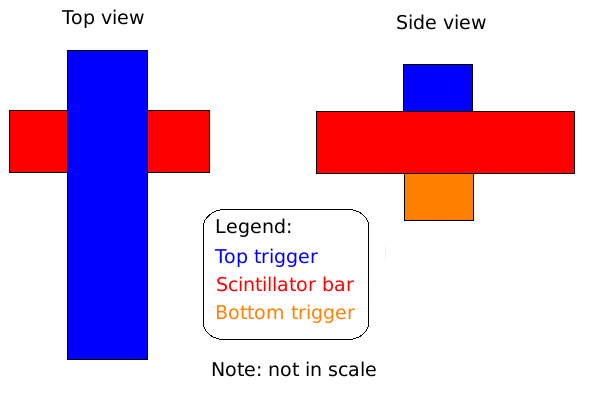
\includegraphics[width=\textwidth]{trigger}
\caption{Sketch of the trigger system}
\label{fig:trigger}
\end{figure}

In this section, channels are the signal from top(bottom) trigger.
These 2 channels enter PS model 740 quad linear FAN IN FAN OUT unit. Its outputs go to PS model 707 16-channels DISCRIMINATOR unit (set at -22.9 mV), whose outputs go to a COINCIDENCE PS model 755 quad four-fold logic unit set as $AND 2$.
Such coincidence have two outputs: one becomes the trigger (after processing of PS model 726 level TRANSLATION LEMO TO ECL), which goes to entry TS#1 of Fastbus; the other output goes through DELAY BOX.
Such delay is +100 ns, then through a PS model 792 DUAL DELAY unit for +8+16+32 on the first module, then the same on the second module. Therefore, the total delay is +100 (box) + (8+16+32)*2 (module) = 212 ns.
The signal, then, goes to a coincidence (aforementioned PS model 755 quad four-fold logic unit) set as $AND 2$. The other input comes from busy from Fastubus. The output of the coincidence undergoes TRANSLATION LEMO TO ECL (via aforementioned PS model 726) and becomes ADC GATE.
After an additional +300 ns delay through the DELAY BOX, ADC GATE outputs TDC GATE. Both GATES go to the ATC CARD in the back of Fastbus.
There are four ECL inputs to this card. The top one is TDC STOP IN. The third one from top (or second from the bottom) is ADC STOP IN. Polarity is such that negative is on top.


\section{Measures for commissioning *EDITED*}\label{sec:meas}

The commissioning of this module requires measures of (ADC) amplitudes and time differences (leading - trailing edge) for signals from cosmic rays.

In particular, we are interested in the following items:
\begin{itemize}
\item selection of horizontal and vertical tracks via cuts;
\item efficiency of said cuts for vertical tracks;
\item leading - trailing edge times;
\item walk correction (ADC vs time difference);
\item frequency of noise.
\end{itemize}

Note that at the moment only one scintillator bar (and the corresponding PMT) is used, so, with the geometrical setup described in section \ref{sec:trig}, the majority of ''true'' (i.e. not background) trigger events comes from almost-vertical tracks as opposed to almost-horizontal tracks.

\subsection{Numbering of ADC and TDC units}
As said in section \ref{sec:geom}, the signals from the scintillators are ultimately sent to ADC and TDC units.
Such units are distinguished by the slot number they occupy.
The physical slot numbers in the crates are mapped, for both ADC and TDC units, into logical slot numbers which start from 0. ADC slot 0 and TDC slot 0 correspond to different physical slot numbers.

The particular units used have 64 channels (ADC) and 96 channels (TDC); analogously to the slot numbers, every input channel for a given unit has an index which starts from 0.

\textbf{EDIT BEGIN}:

\subsection{Horizontal and vertical tracks}\label{sec:tracks}
TODO
See figures \ref{fig:tracks}, \ref{fig:horizontal}, \ref{fig:peak}.

\begin{figure}[htbp]
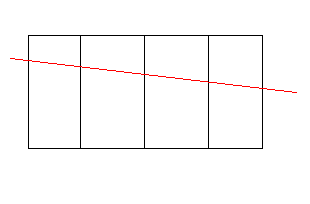
\includegraphics[width=0.5\textwidth]{horizontal}%
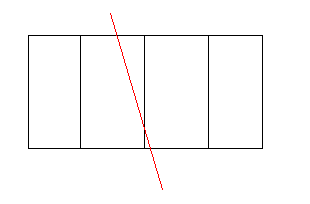
\includegraphics[width=0.5\textwidth]{vertical}
\caption{The black box represents a few contiguous sensible elements in a scintillator bar. 
In the left figure, the red line is an example of (nearly) horizontal track. In this case, all the blocks output a relatively high ADC amplitude.
In the right figure, the red line is an example of (nearly) vertical track. In this case, only one block of the series outputs a relatively high ADC amplitude.}
}
\label{fig:tracks}
\end{figure}

\begin{figure}[htbp]
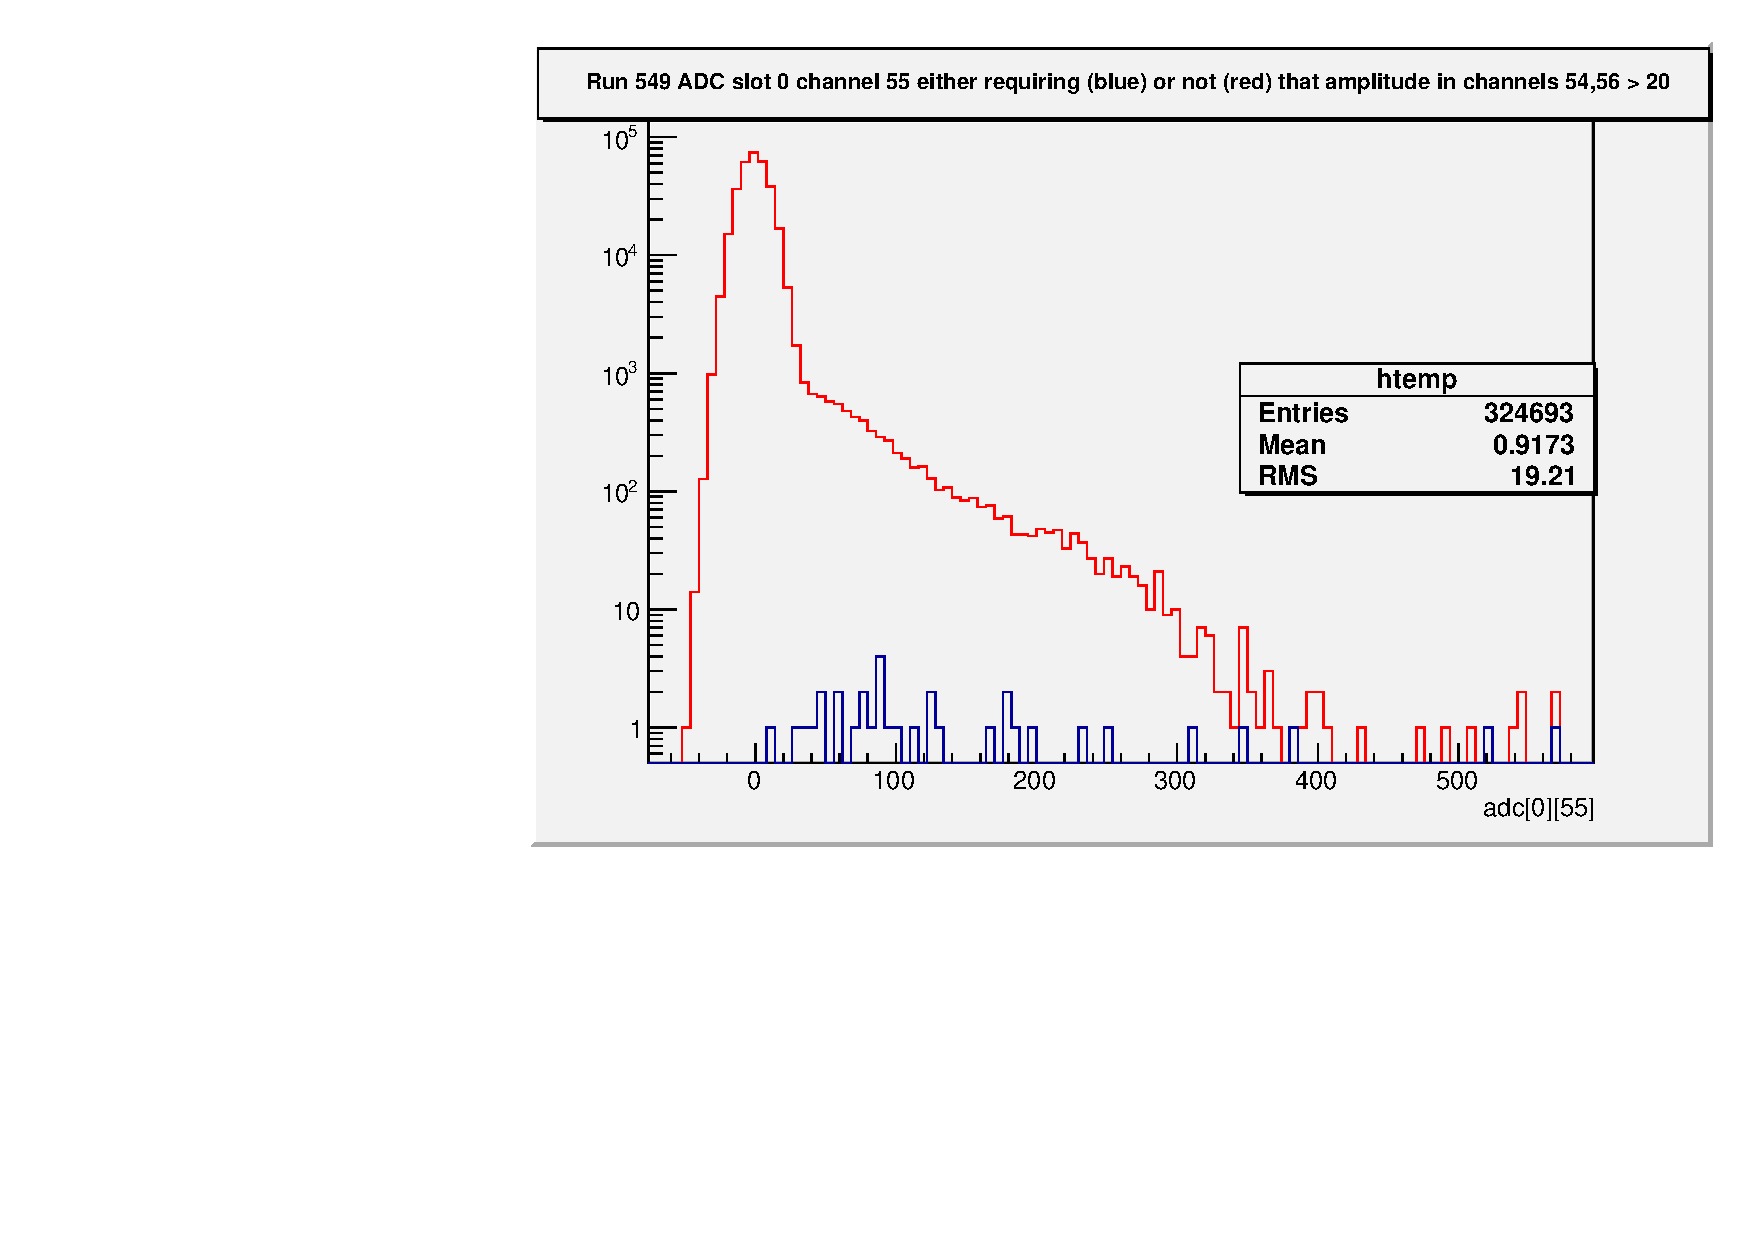
\includegraphics[width=\textwidth]{run_549_horizontal_cut20_55}
\caption{Example of selection of horizontal track. Red histogram represents ADC amplitude (run 549, slot 0, channel 55) distribution without cuts, blue histogram is the previous one after the request that the immediate neighbors have at least amplitude 20.}
\label{fig:horizontal}
\end{figure}

\begin{figure}[htbp]
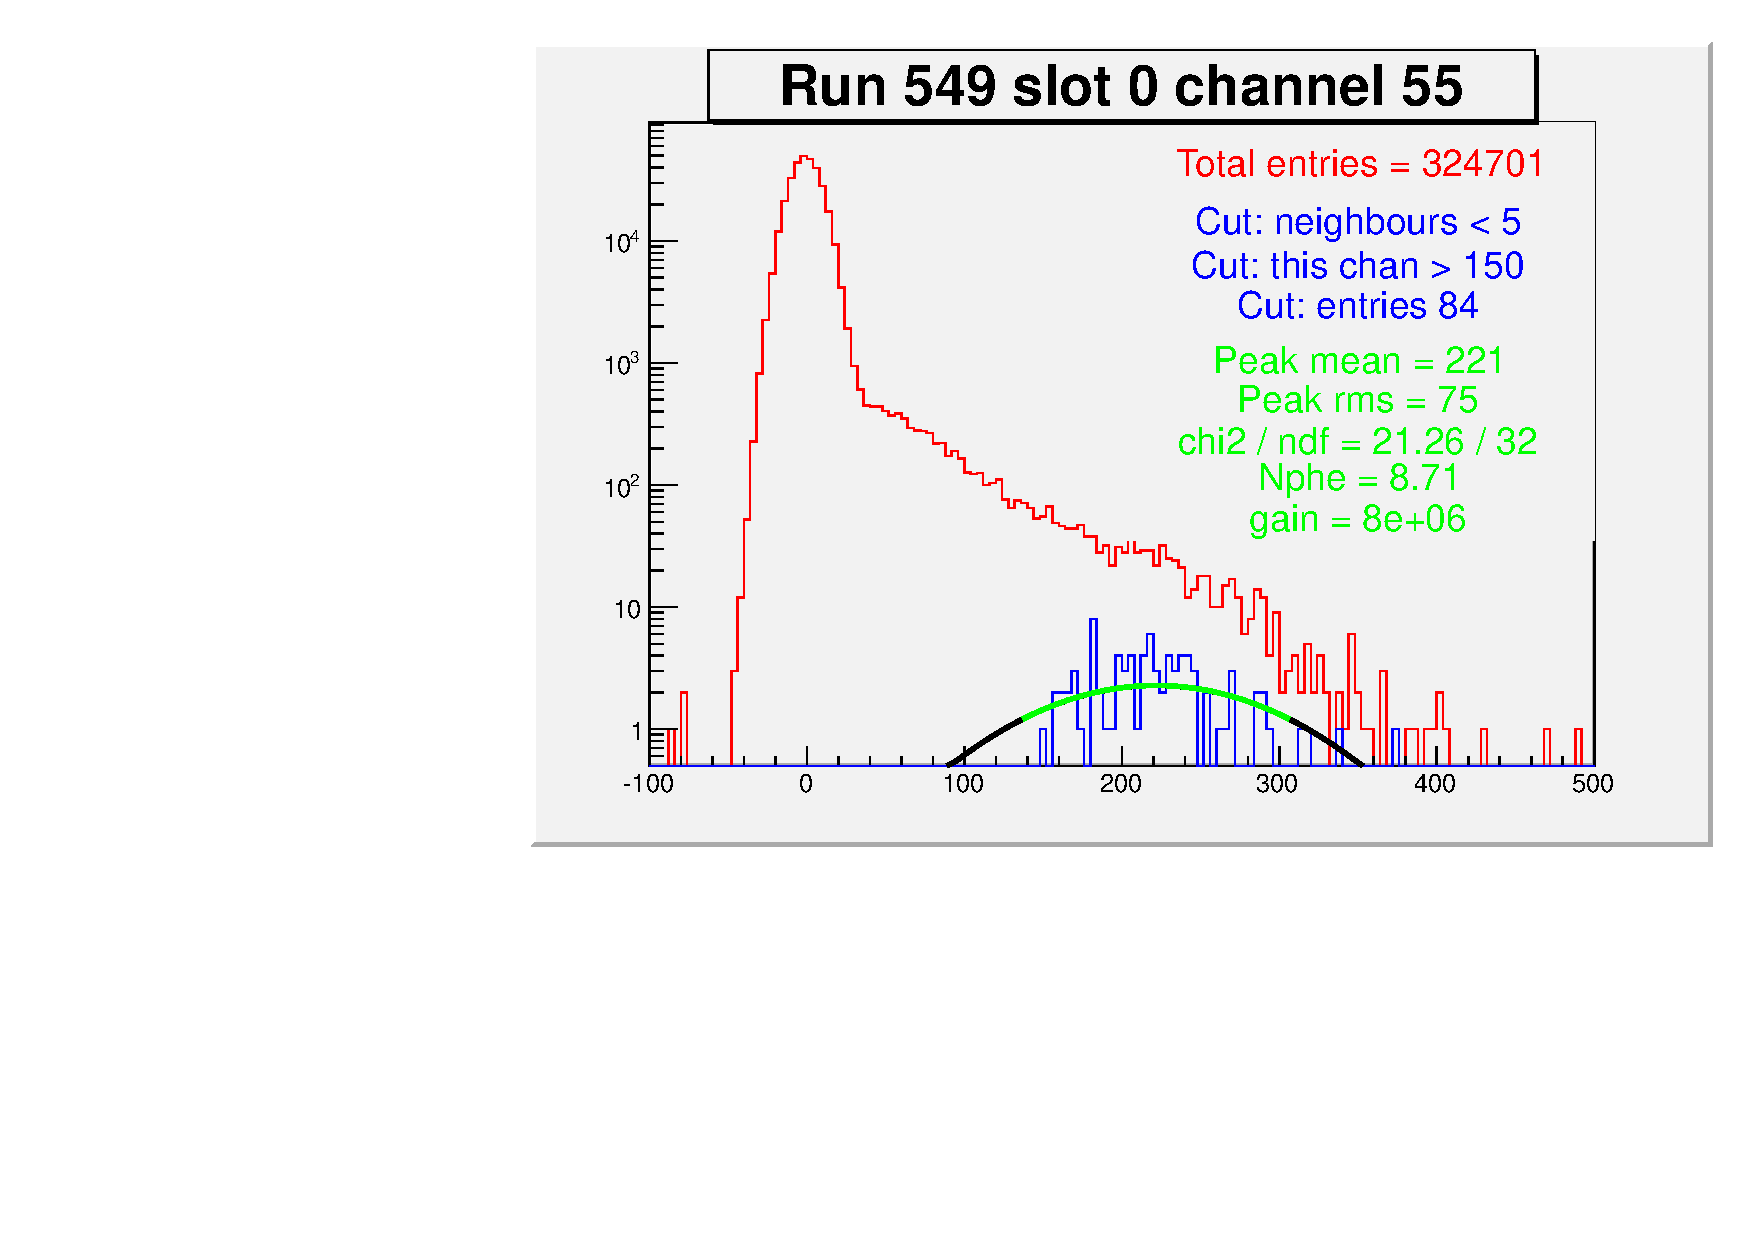
\includegraphics[width=\textwidth]{run_549_peak_55}
\caption{Example of selection of vertical track. Red histogram represents ADC amplitude (run 549, slot 0, channel 55) distribution without cuts, blue peak is the result of requiring that the neighboring channels in the red histogram have amplitude less than 5 and the current channel an amplitude reasonably above pedestal, black line is the best fit of the blue peak, and finally the range used for the fit has been highlighted in green.}
\label{fig:peak}
\end{figure}

phe? What is gain? conclusions

Nphe = (mean/rms)**2
Qphe = mean/Nphe * 50 fC
Gain = Qphe/(1.6e-19 C)

\subsection{Efficiency}\label{sec:eta}
TODO.
See figures \ref{fig:eta_fit}, \ref{fig:eta_adc}.

\begin{figure}[htbp]
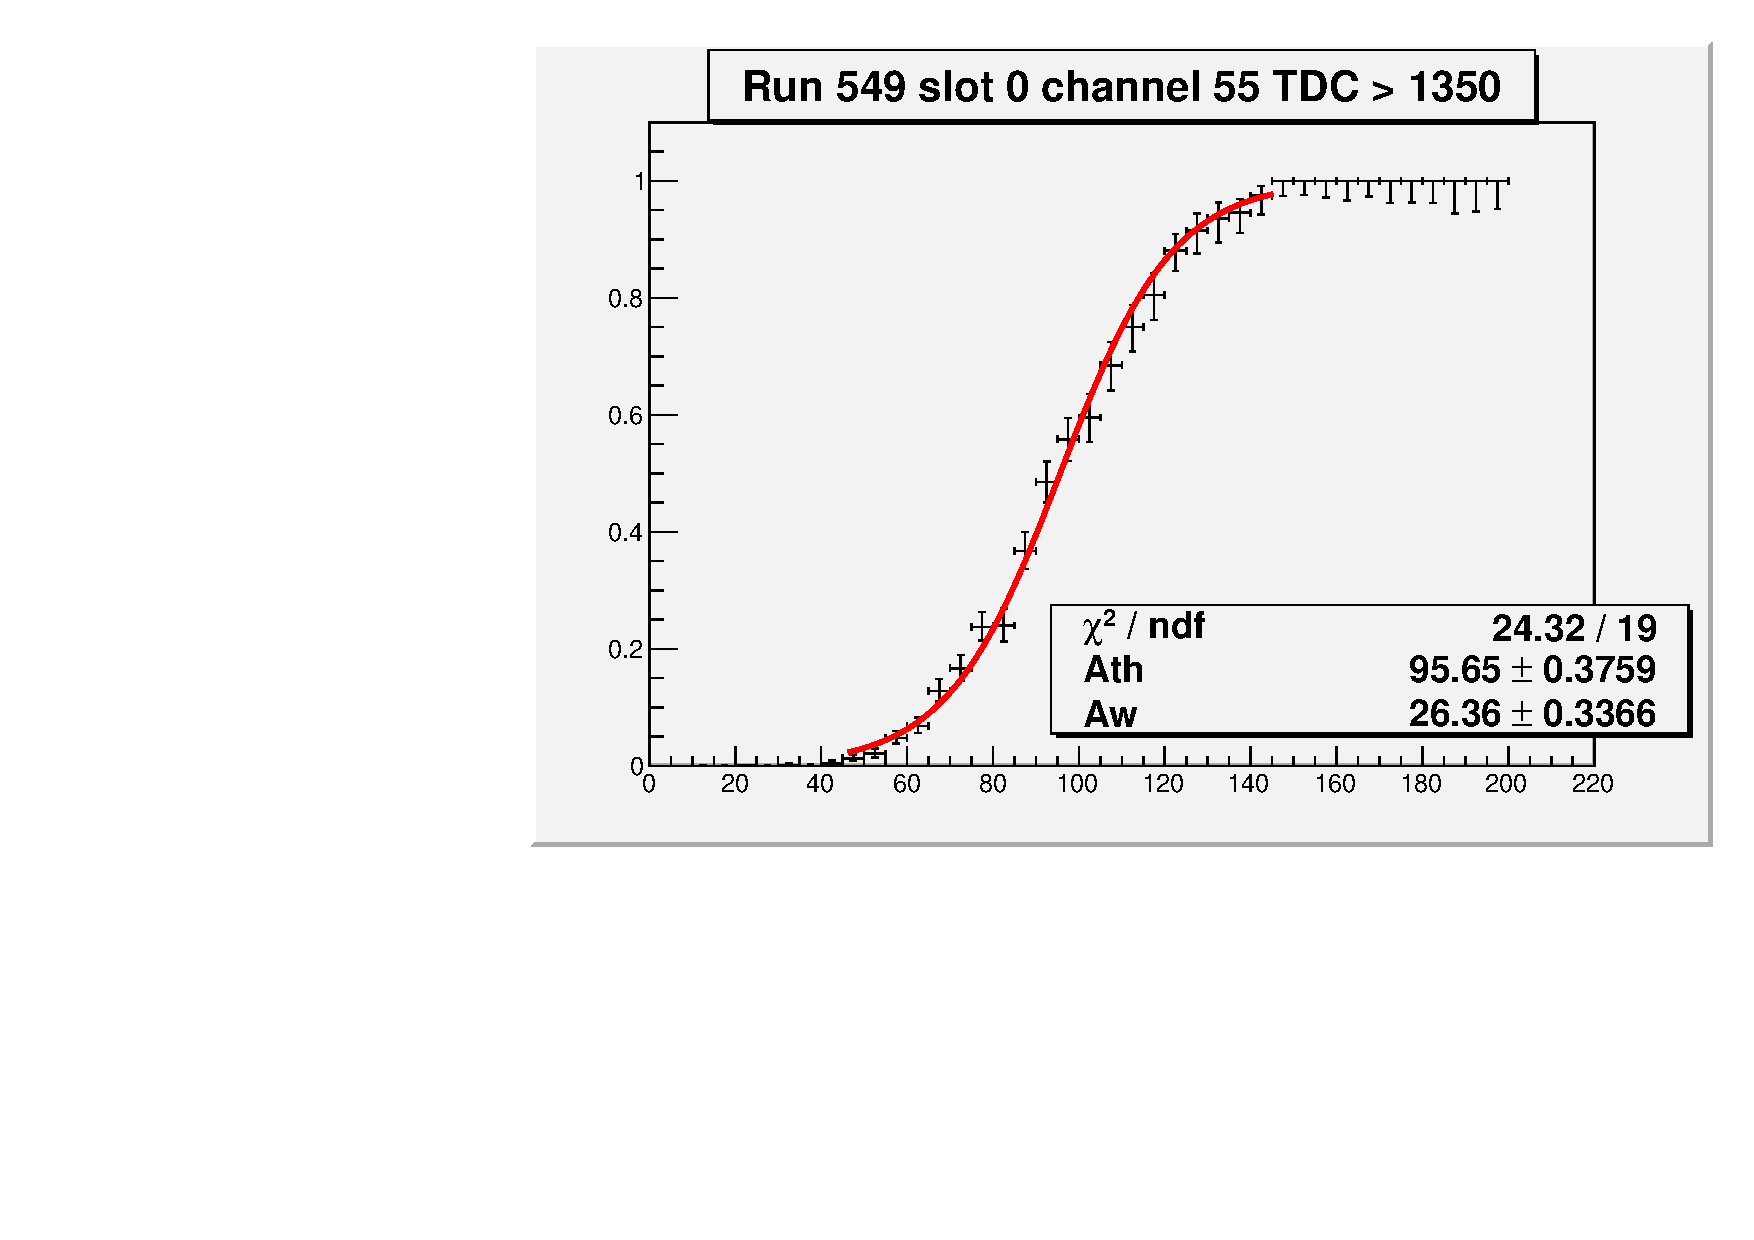
\includegraphics[width=\textwidth]{run_549_eta_55}
\caption{Efficiency (and its fit) for run 549, slot 0, channel 55, using a given cut on TDC. Errors are statistic.}
\label{fig:eta_fit}
\end{figure}

\begin{figure}[htbp]
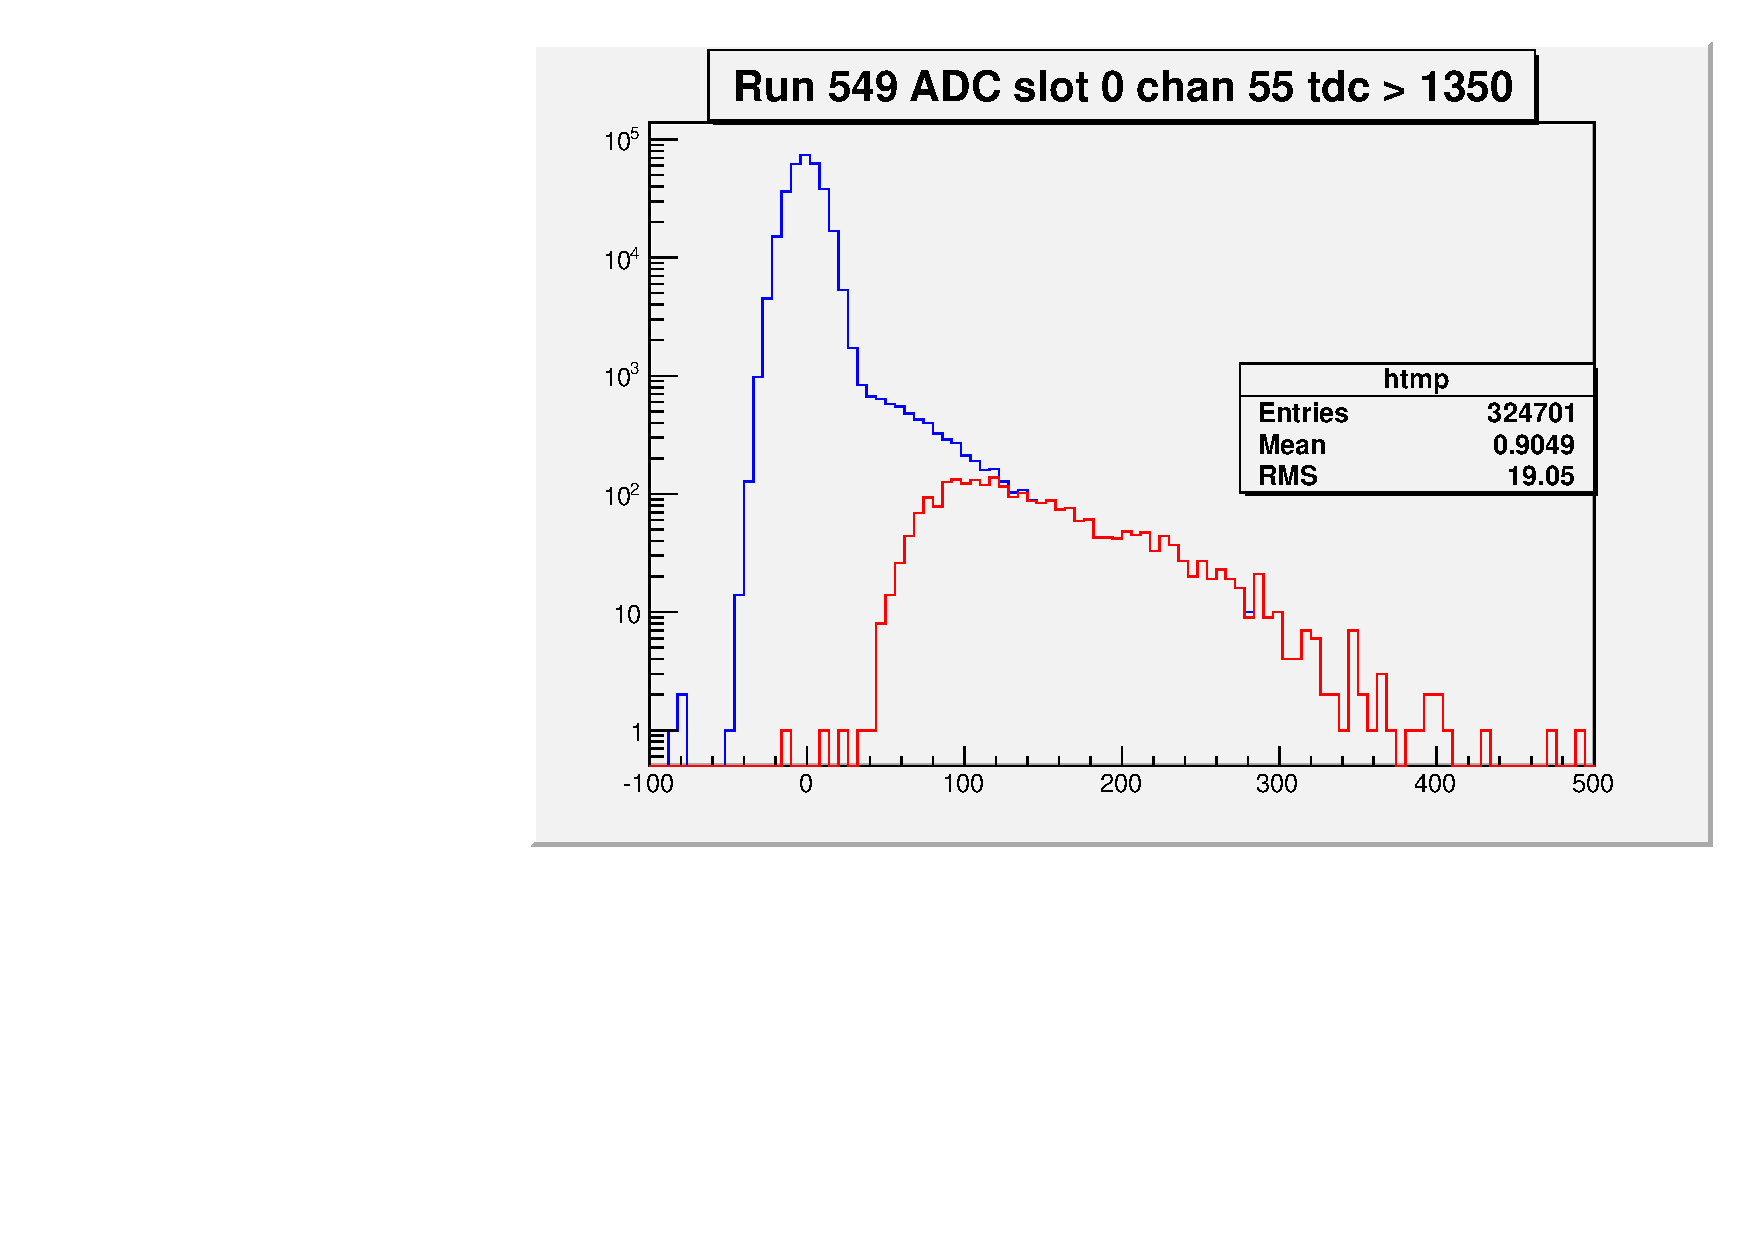
\includegraphics[width=\textwidth]{run_549_adc_55}
\caption{Red (blue) histogram is ADC amplitude for run 549, slot 0, channel 55 with (without) a given cut on TDC.}
\label{fig:eta_adc}
\end{figure}

\subsection{Amplitude vs Voltage}\label{sec:adcv}
TODO.
peak position vs NINO threshold.
See figures \ref{fig:peak_563} and \ref{fig:peak_536}

\begin{figure}[htbp]
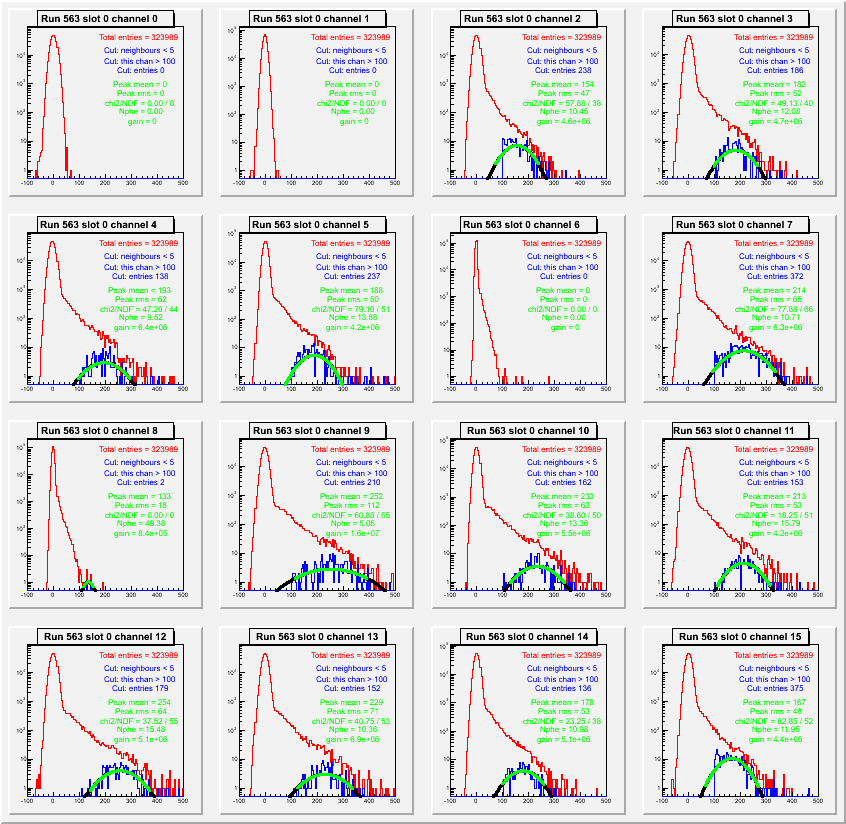
\includegraphics[width=\textwidth]{run_563_peaks_slot_0_chans_0_15_lt_5_gt_100}
\caption{Peak positions for run 563 (NINO threshold -1.4V, HV=700V, 325k events)}
\label{fig:peak_563}
\end{figure}

\begin{figure}[htbp]
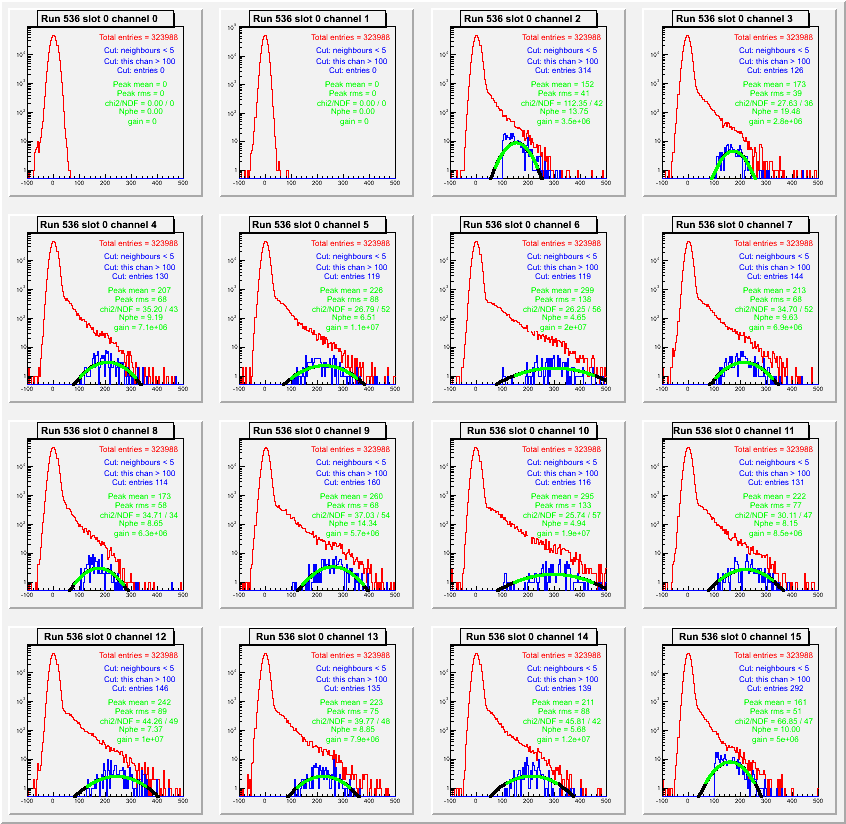
\includegraphics[width=\textwidth]{run_536_peaks_slot_0_chans_0_15_lt_5_gt_100}
\caption{Peak positions for run 536 (NINO threshold -1.9V, HV=700V, 325k events)}
\label{fig:peak_536}
\end{figure}

\subsection{Leading - Trailing edge times}\label{sec:dtime}
TODO.


%\begin{figure}[htbp]
%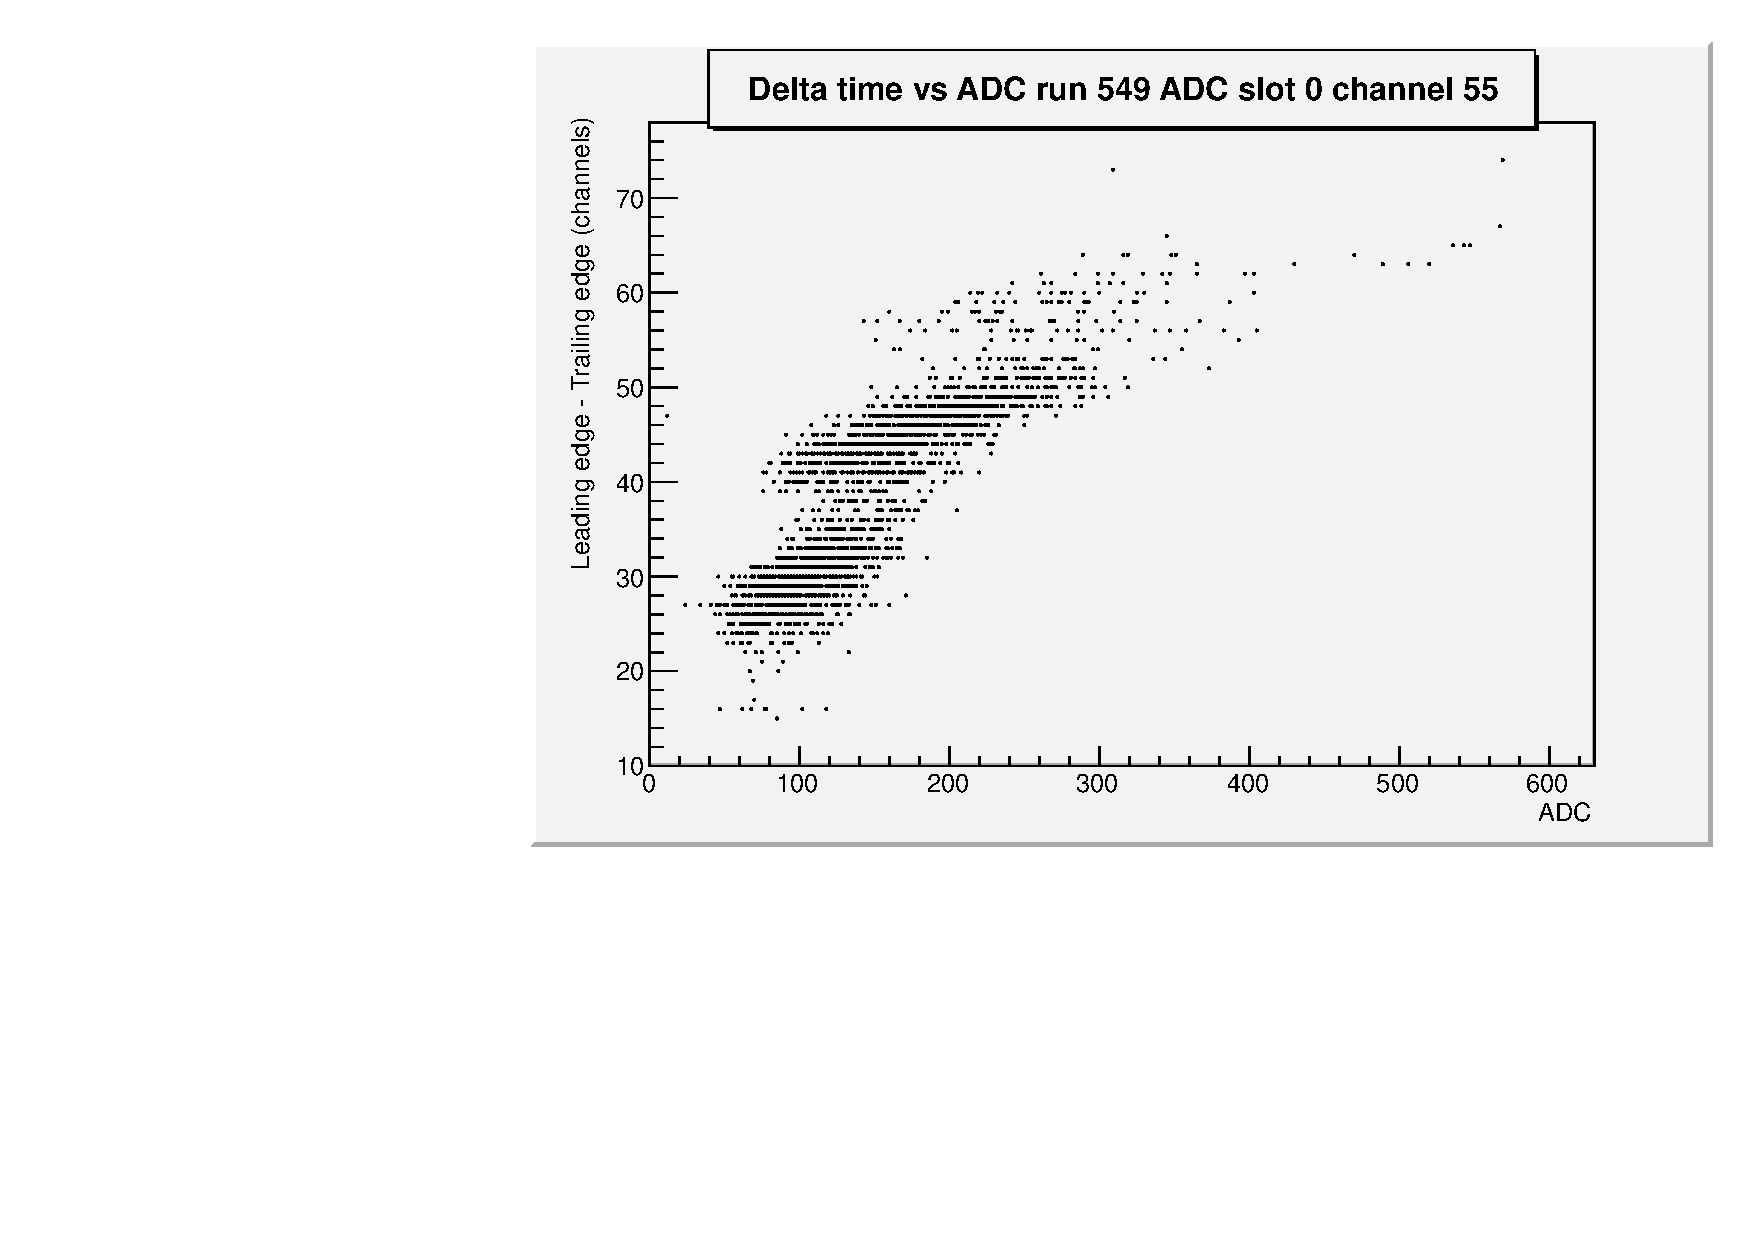
\includegraphics[width=\textwidth]{run_549_deltat_vs_adc_55}
%\caption{On the vertical axis the $\Delta$t, and on the horizontal axis the ADC amplitude for run 549, slot 0, channel 55. Pedestal ends at about bin 80}
%\label{fig:dt_adc}
%\end{figure}


Walk correction (ADC vs time difference); see figure \ref{fig:walk_stages}, \ref{fig:walk}.

\begin{figure}[htbp]
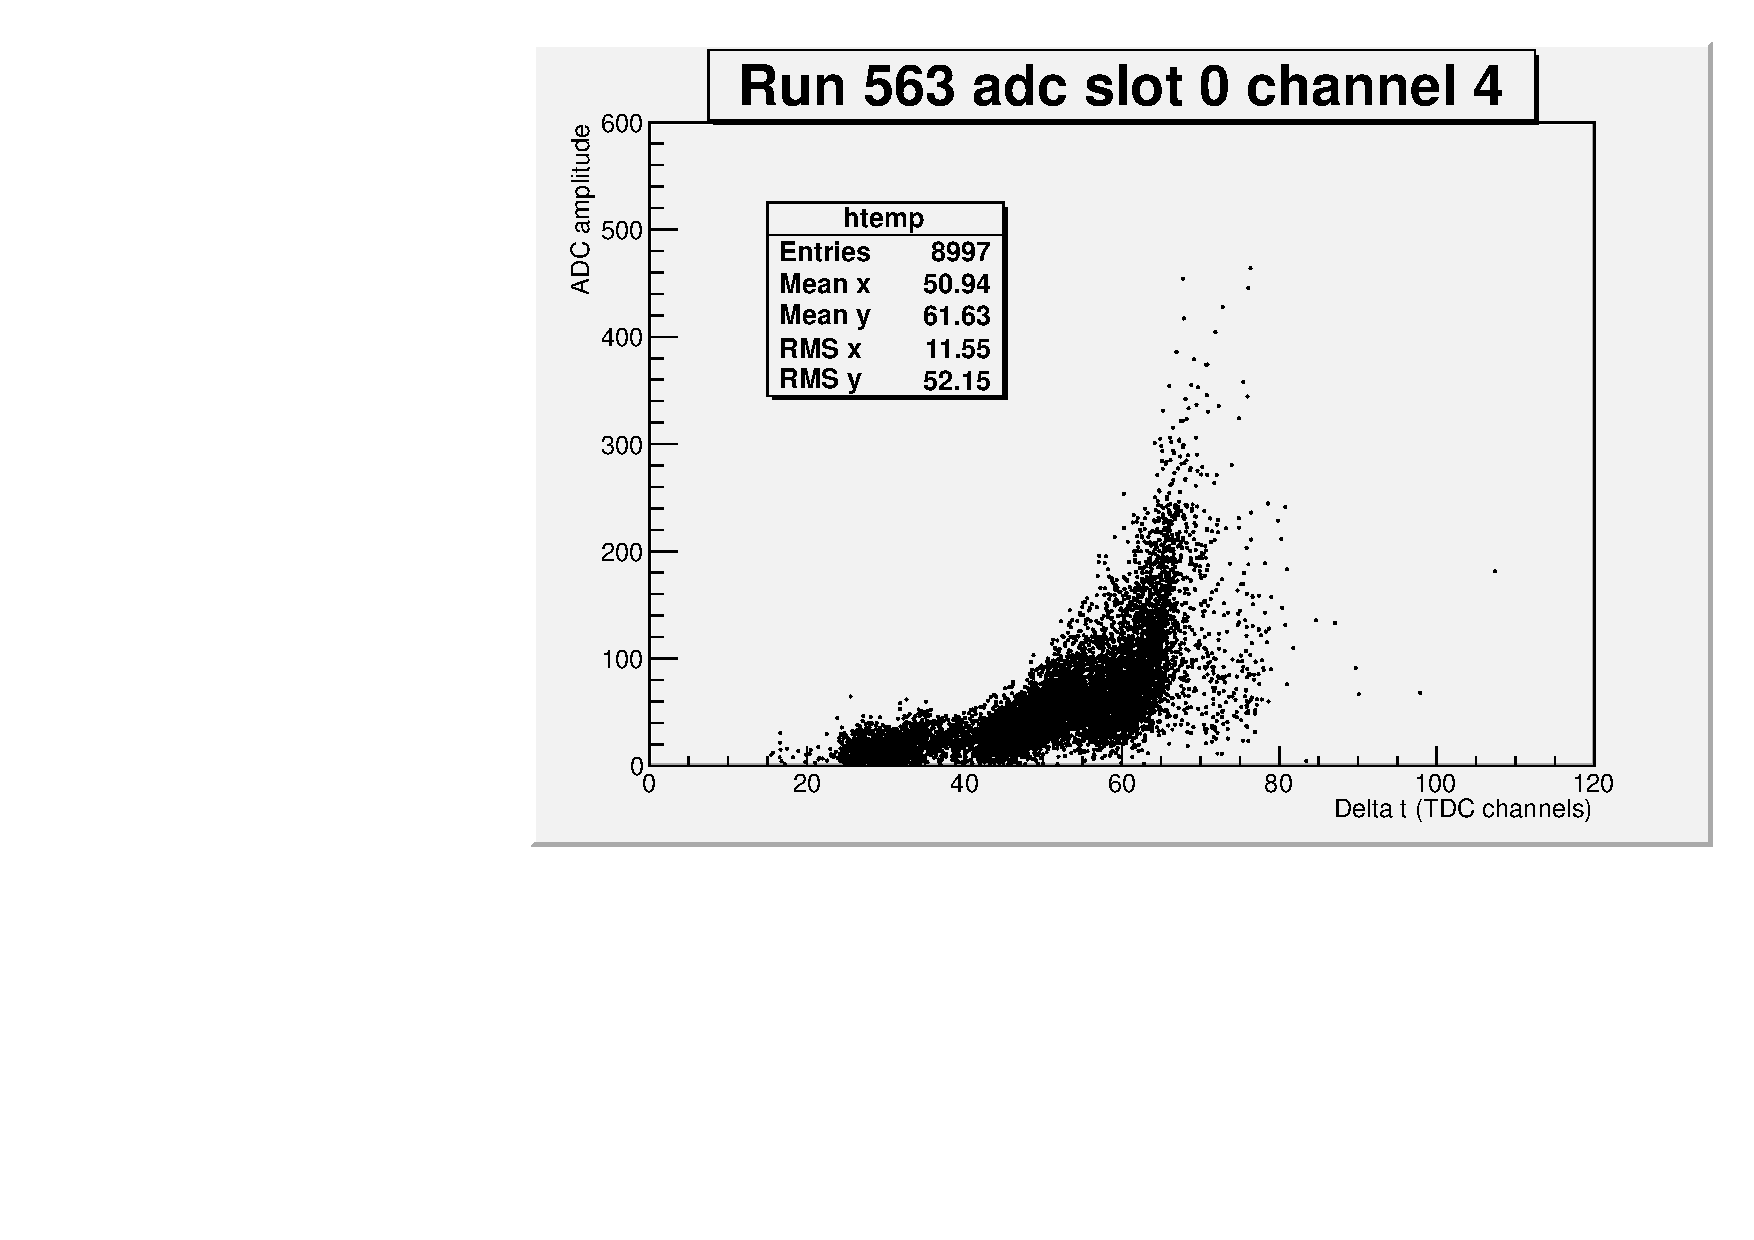
\includegraphics[width=0.5\textwidth]{walk_stage1}%
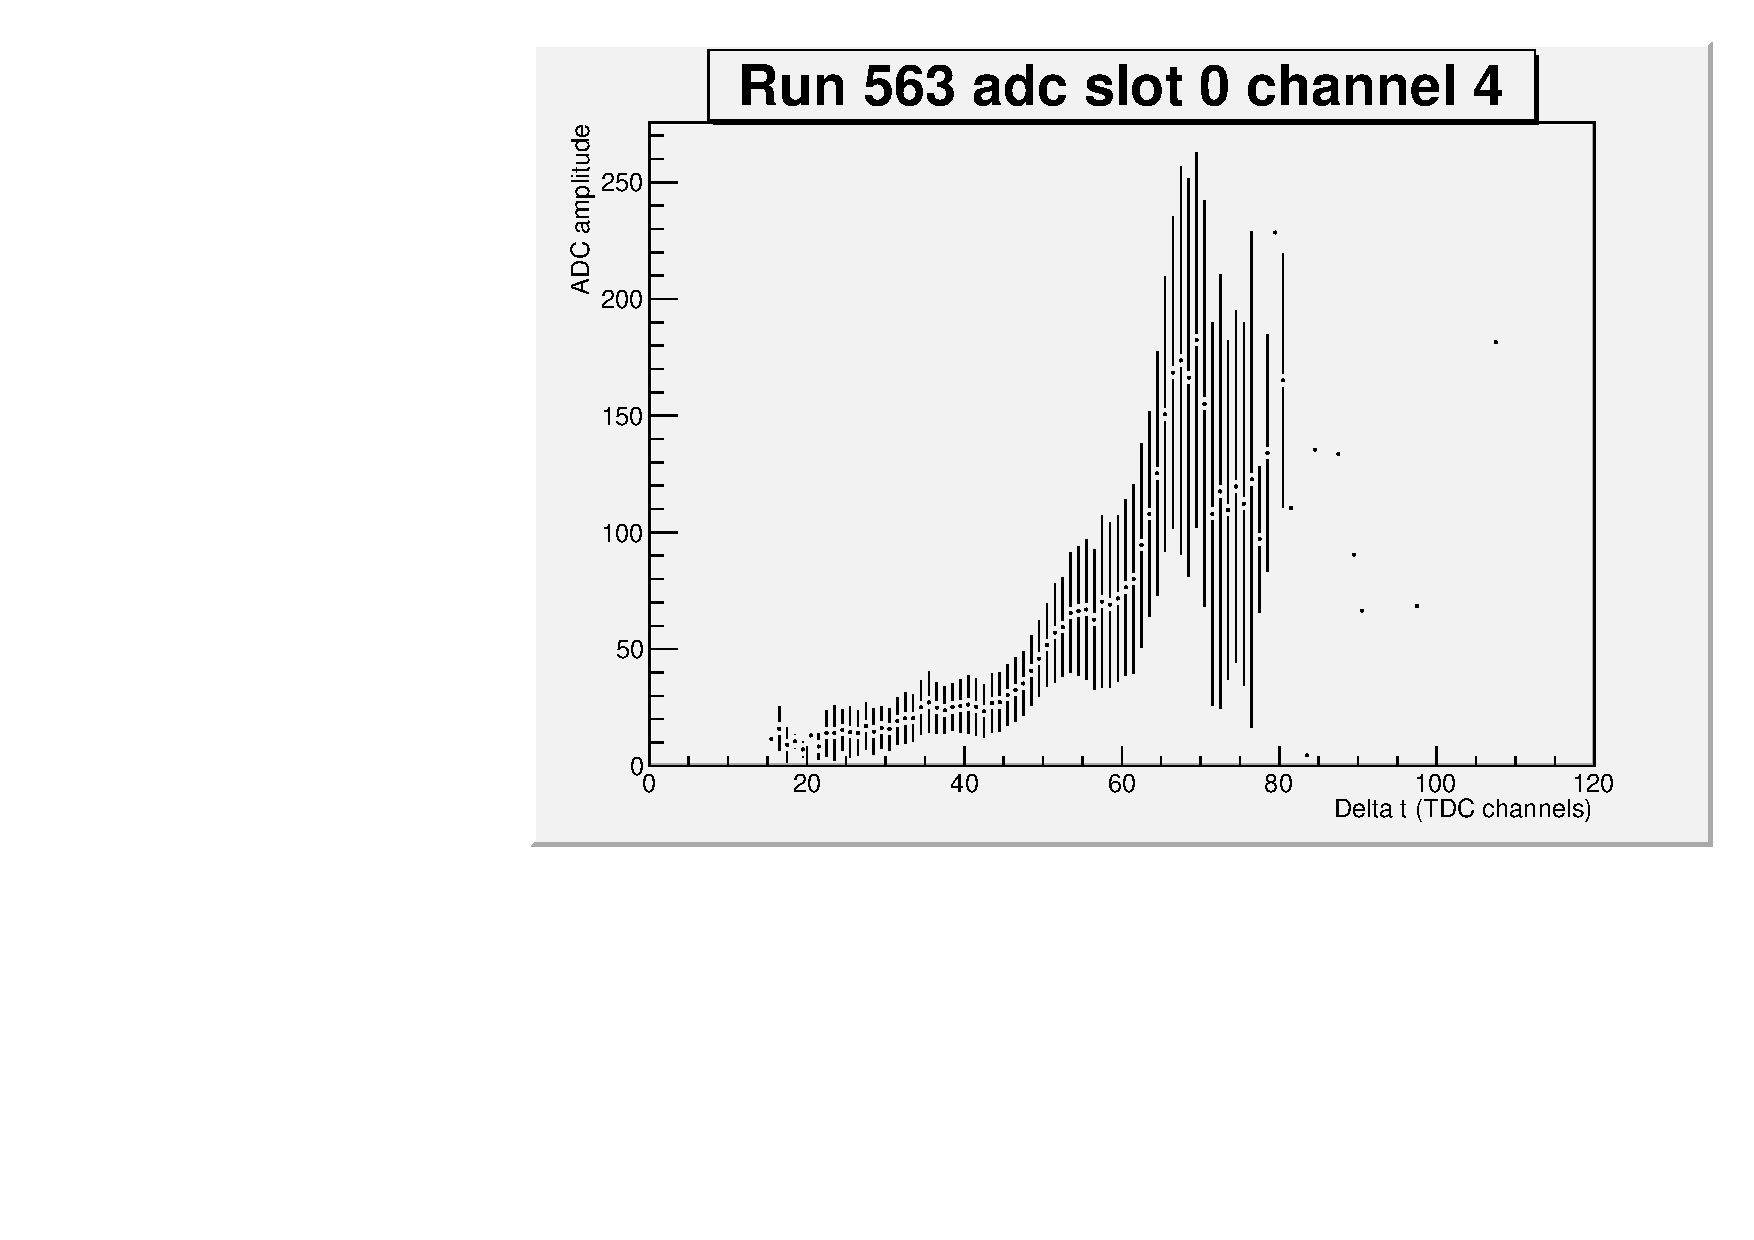
\includegraphics[width=0.5\textwidth]{walk_stage2}\\
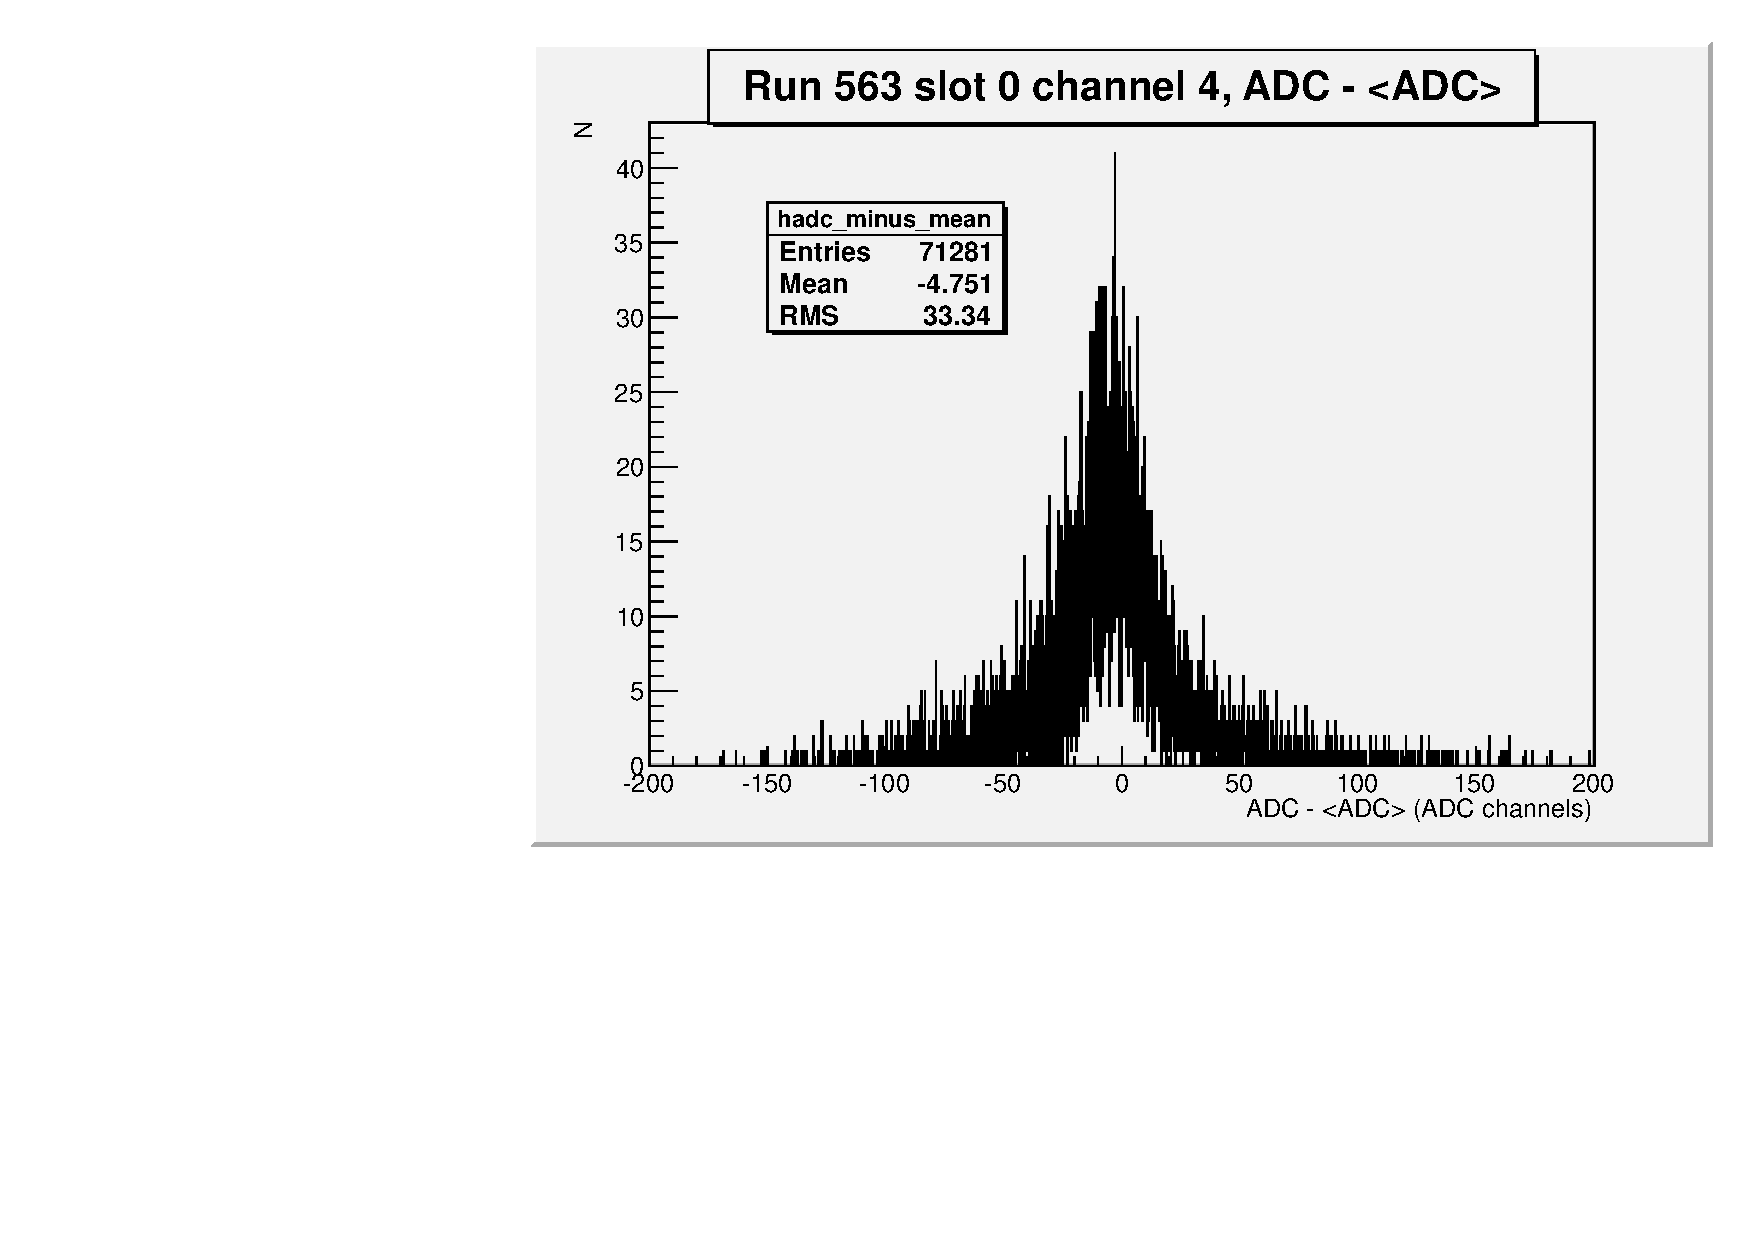
\includegraphics[width=0.5\textwidth]{walk_stage3}%
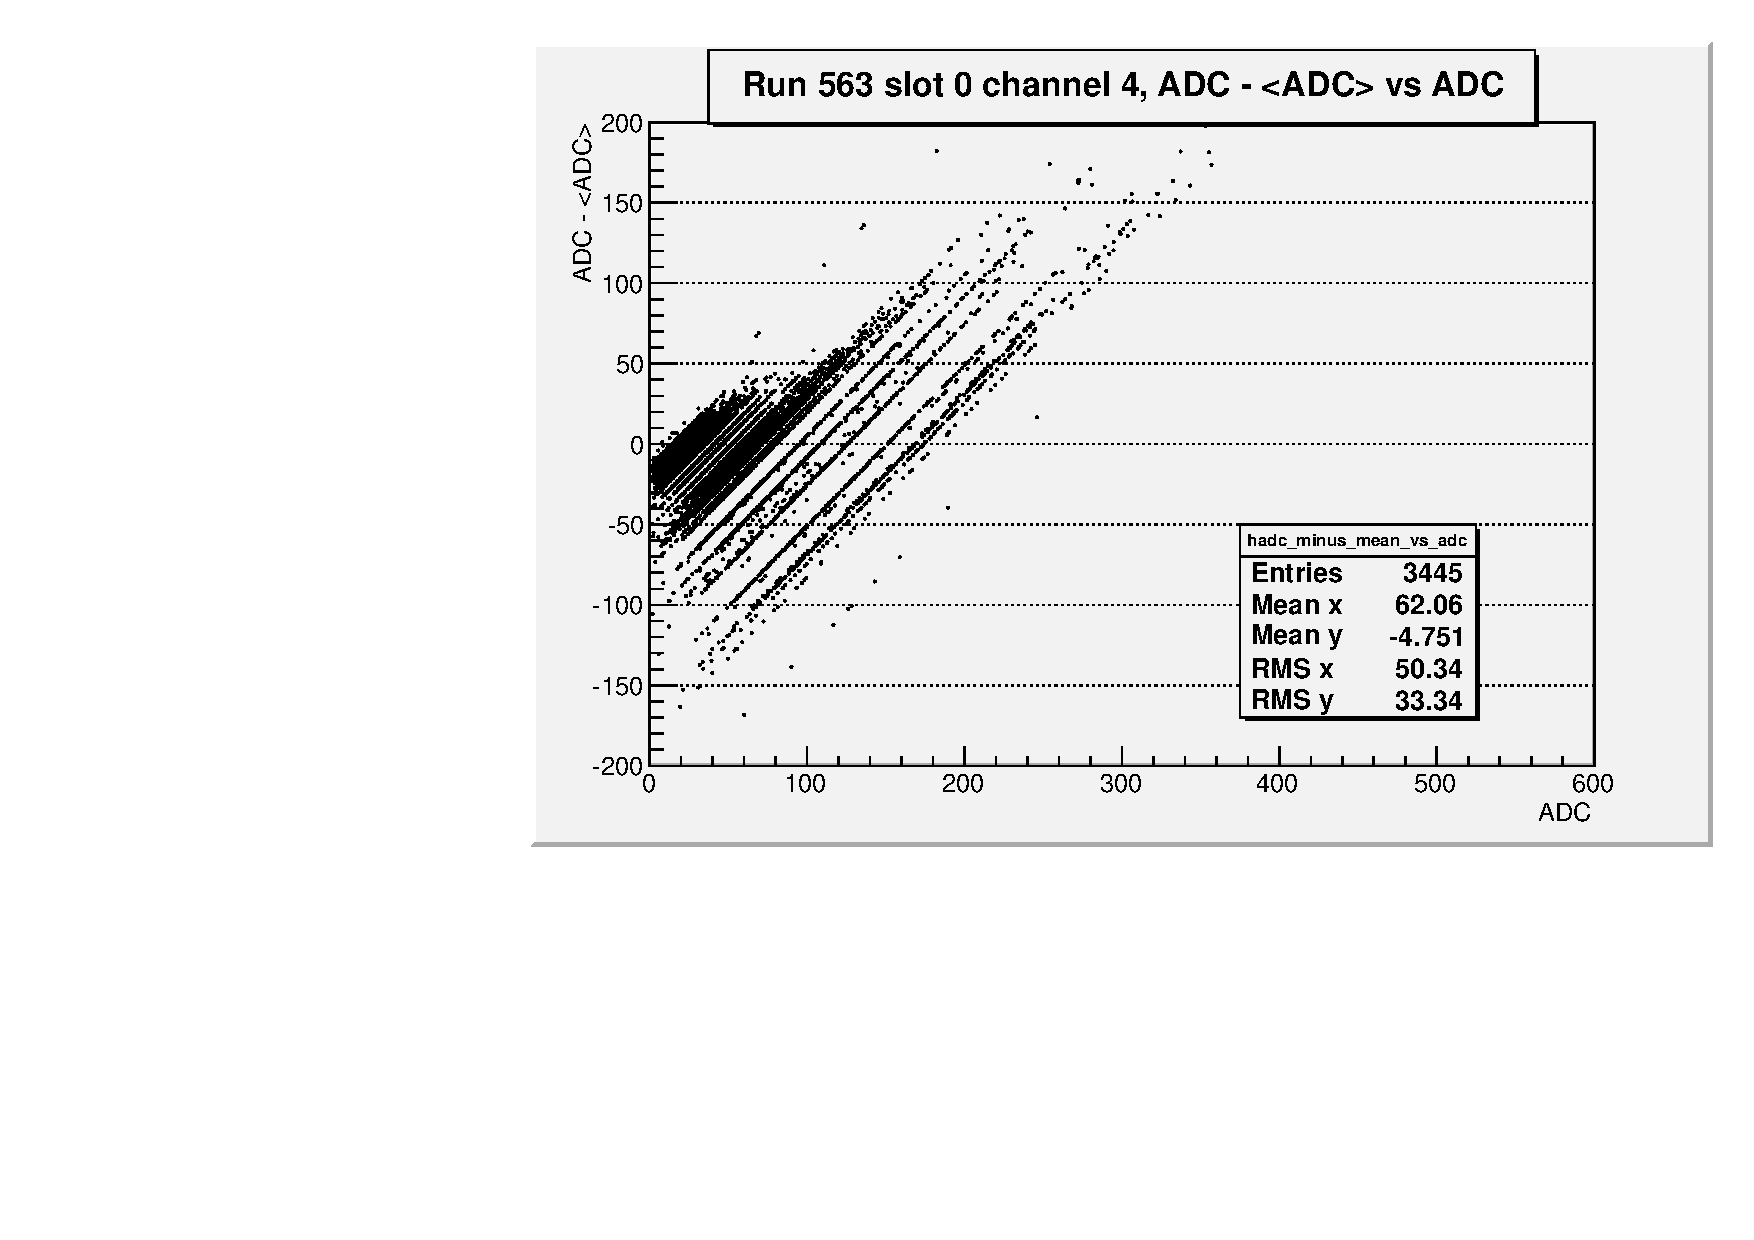
\includegraphics[width=0.5\textwidth]{walk_stage4}\\
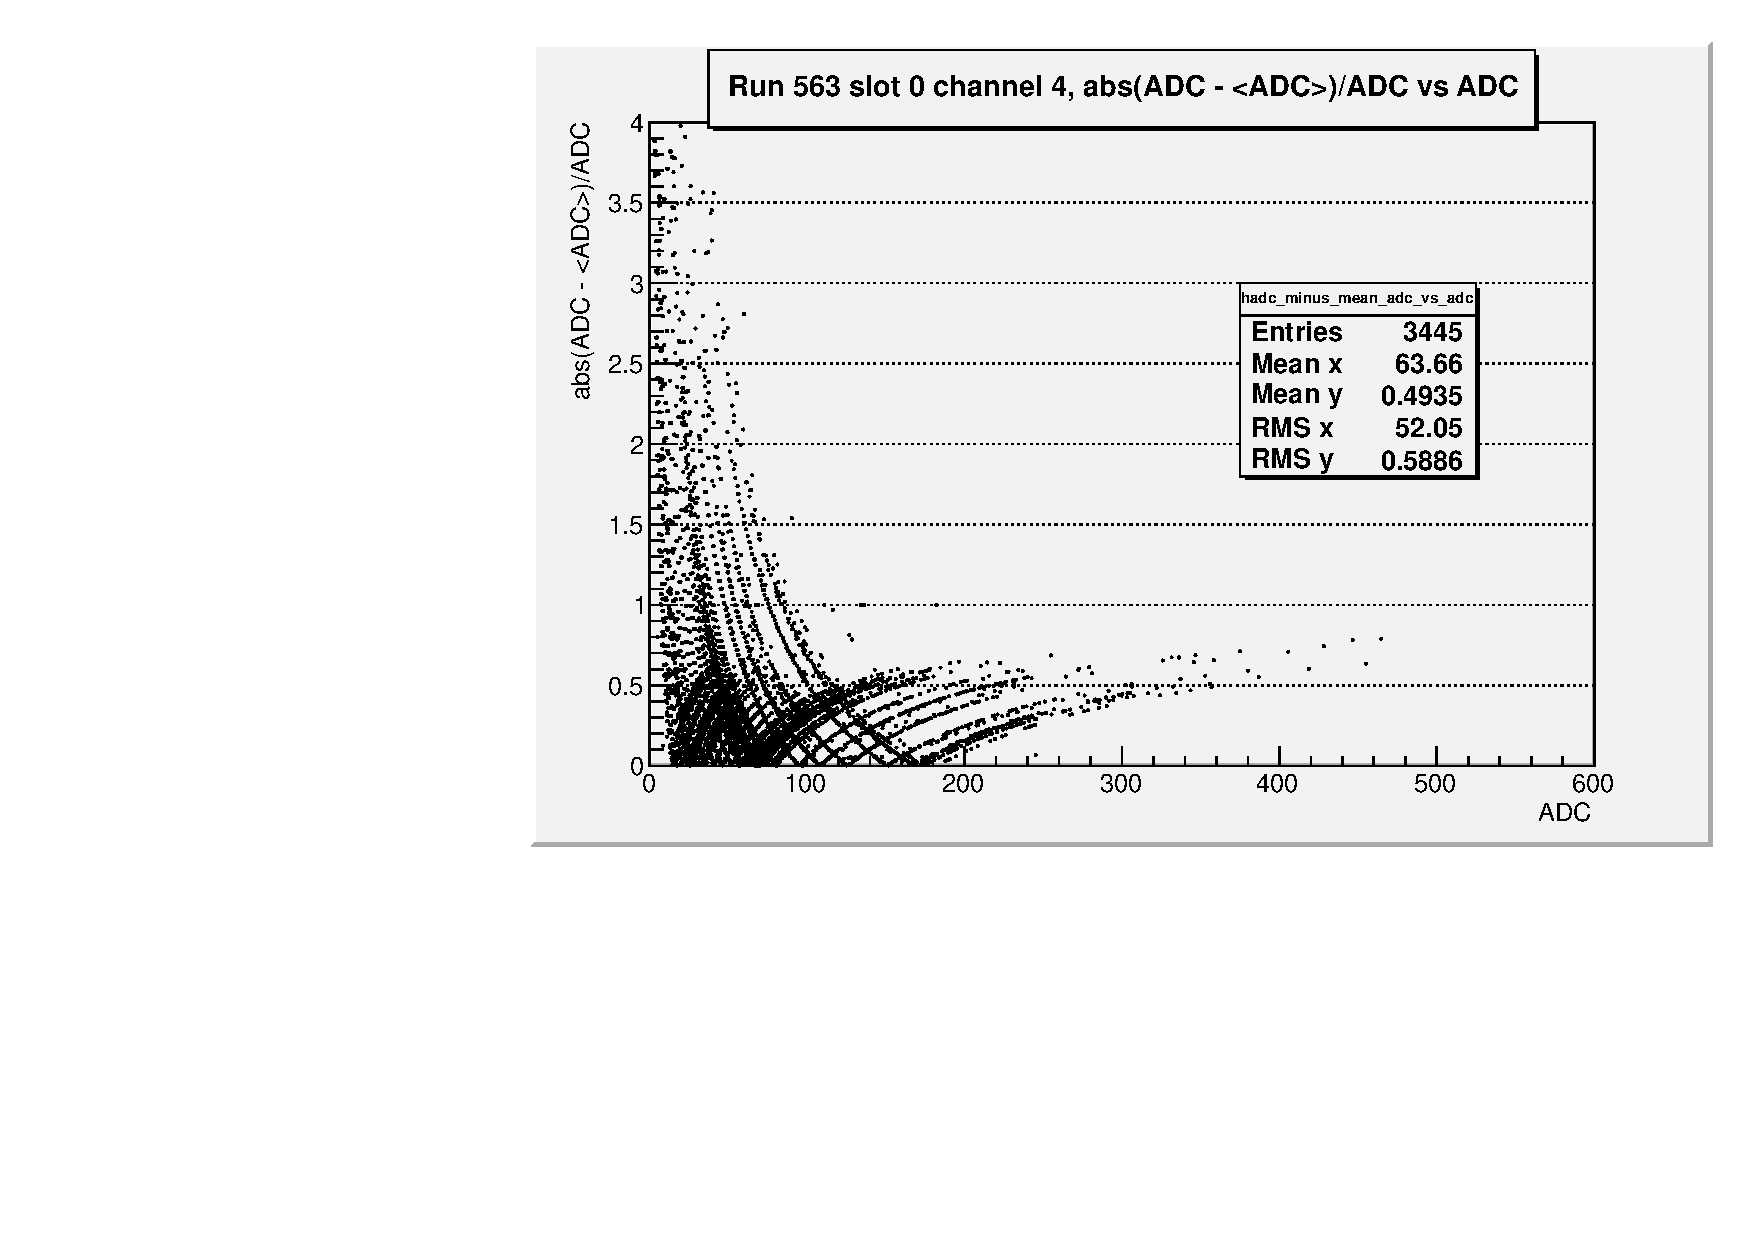
\includegraphics[width=0.5\textwidth]{walk_stage5}%
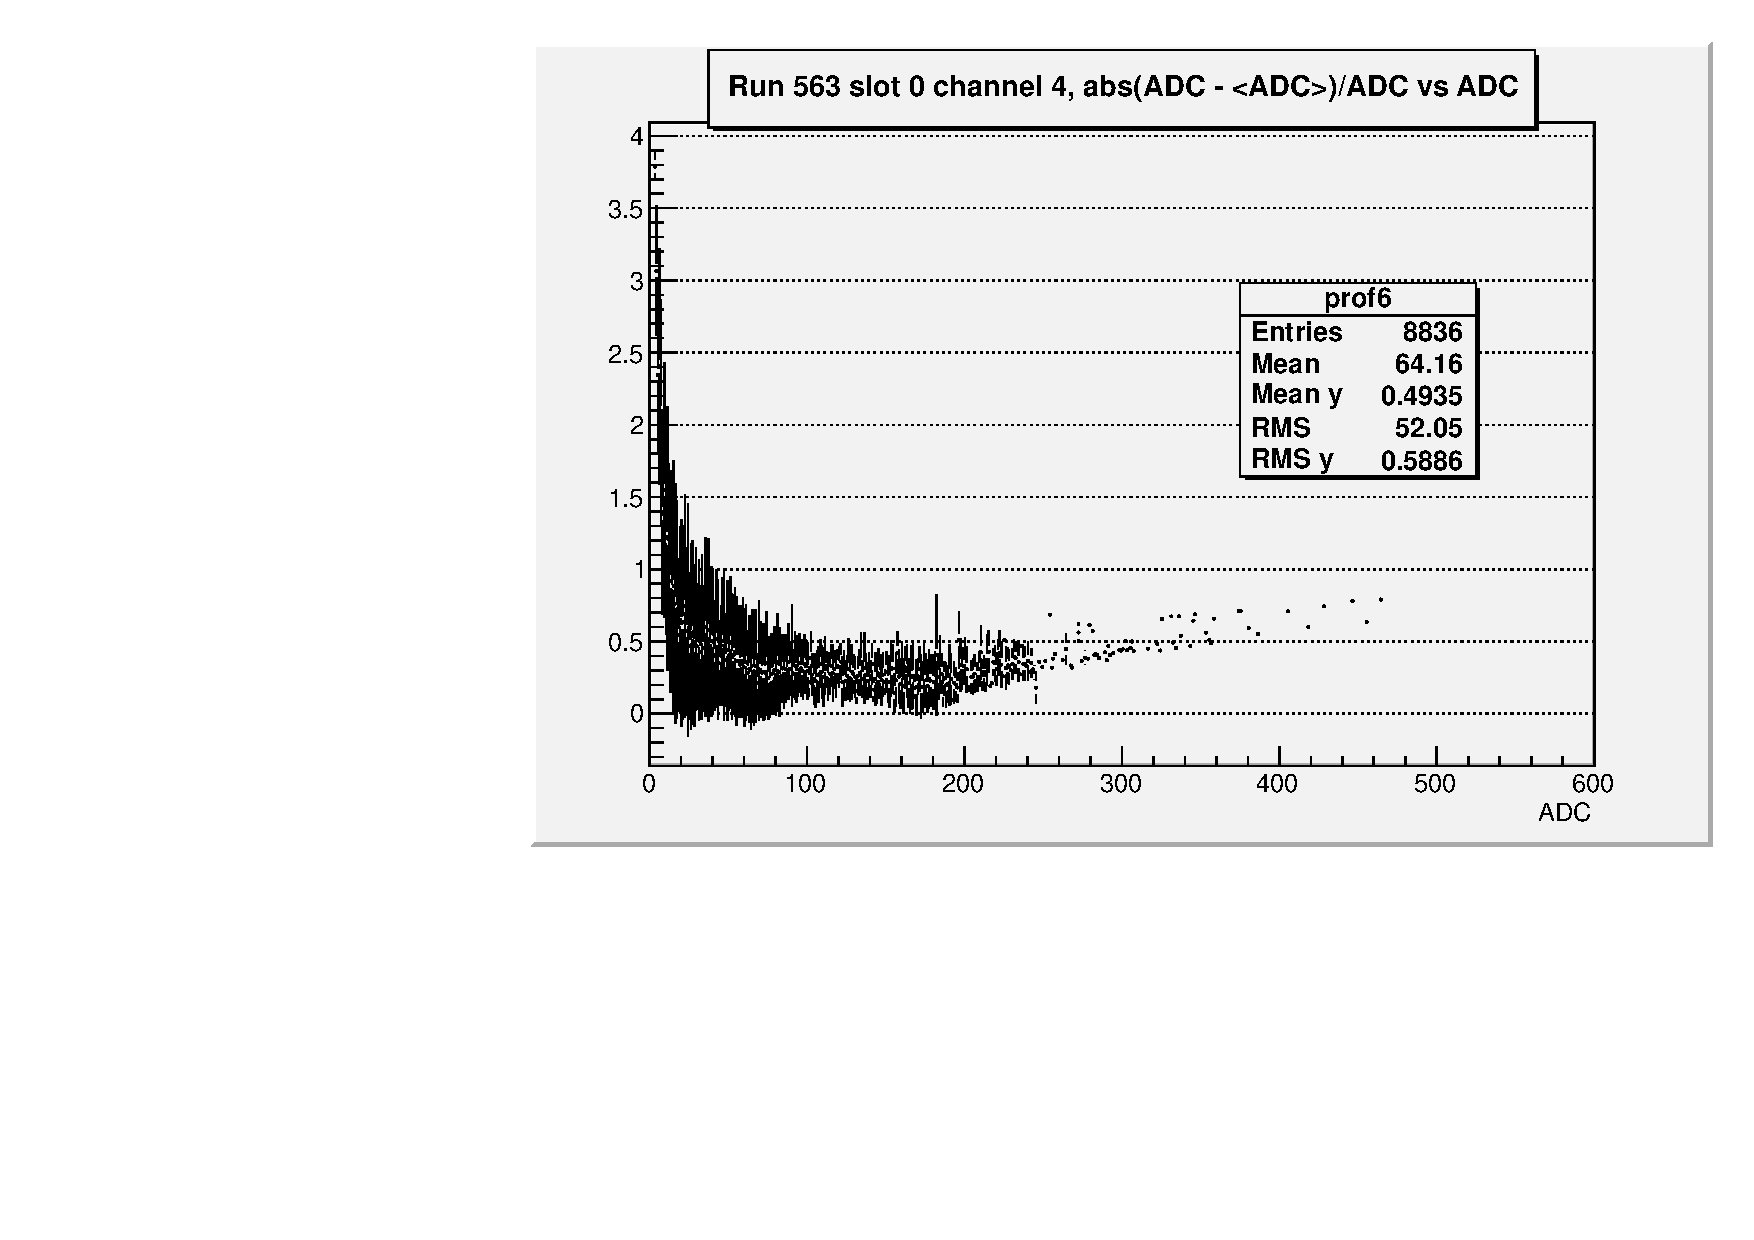
\includegraphics[width=0.5\textwidth]{walk_stage6}
\caption{Example of calculation of walk. Stages are presented left to right, top to bottom.
Stage 1: ADC vs $\Delta t$.
Stage 2: X-profile histogram of Stage 1: for a given bin in the horizontal axis (i.e $\Delta t$), points are averages of ADC values with $Delta t$ in the chose bin, error bar is their RMS.
Stage 3: Check that $ADC - <ADC>$ has a symmetric distribution around 0.
Stage 4: $ADC - <ADC>$ versus ADC.
Stage 5: relative error $abs(ADC - <ADC>)/ADC$ versus ADC.
Stage 6: X-profile of stage 5.}
\label{fig:walk_stages}
\end{figure}

\begin{figure}[htbp]
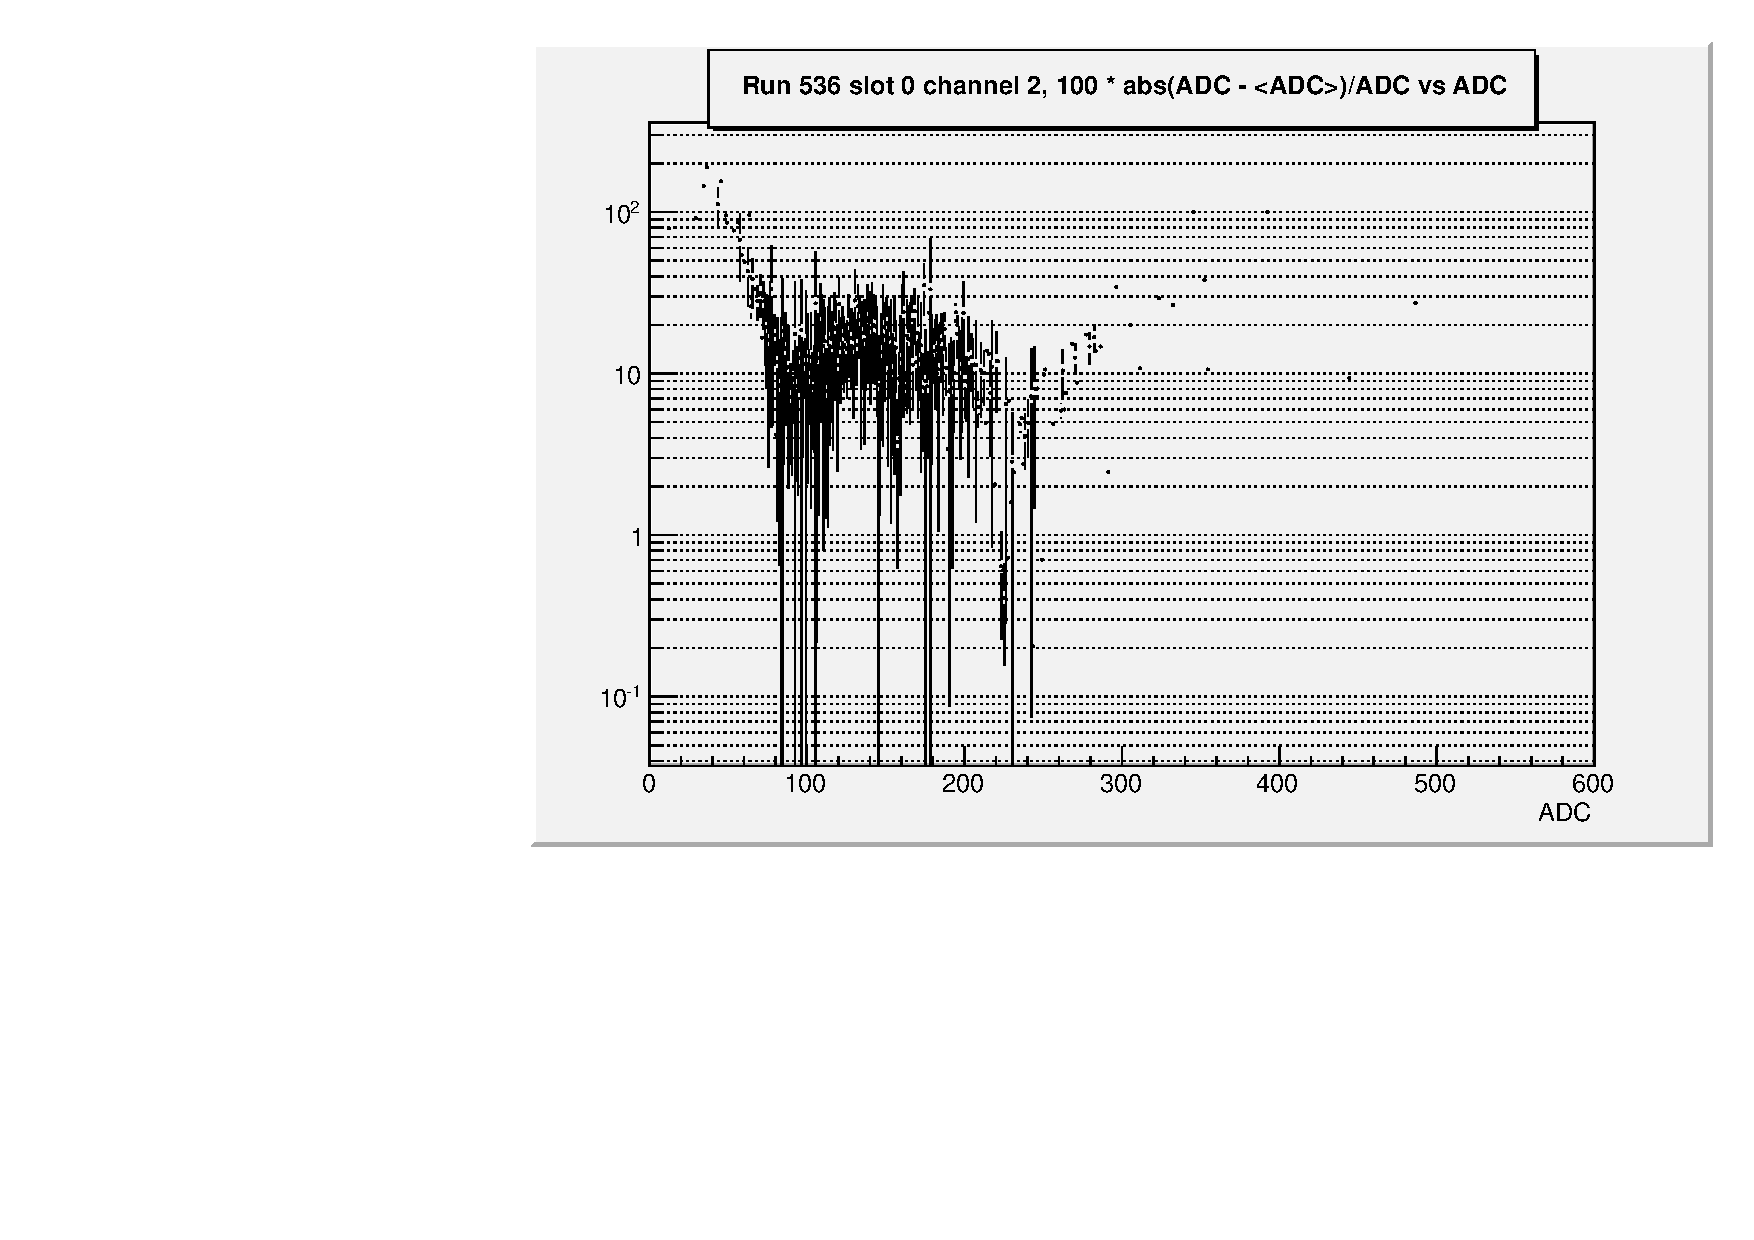
\includegraphics[width=\textwidth]{walk_NINO_1_9_PMT_700}
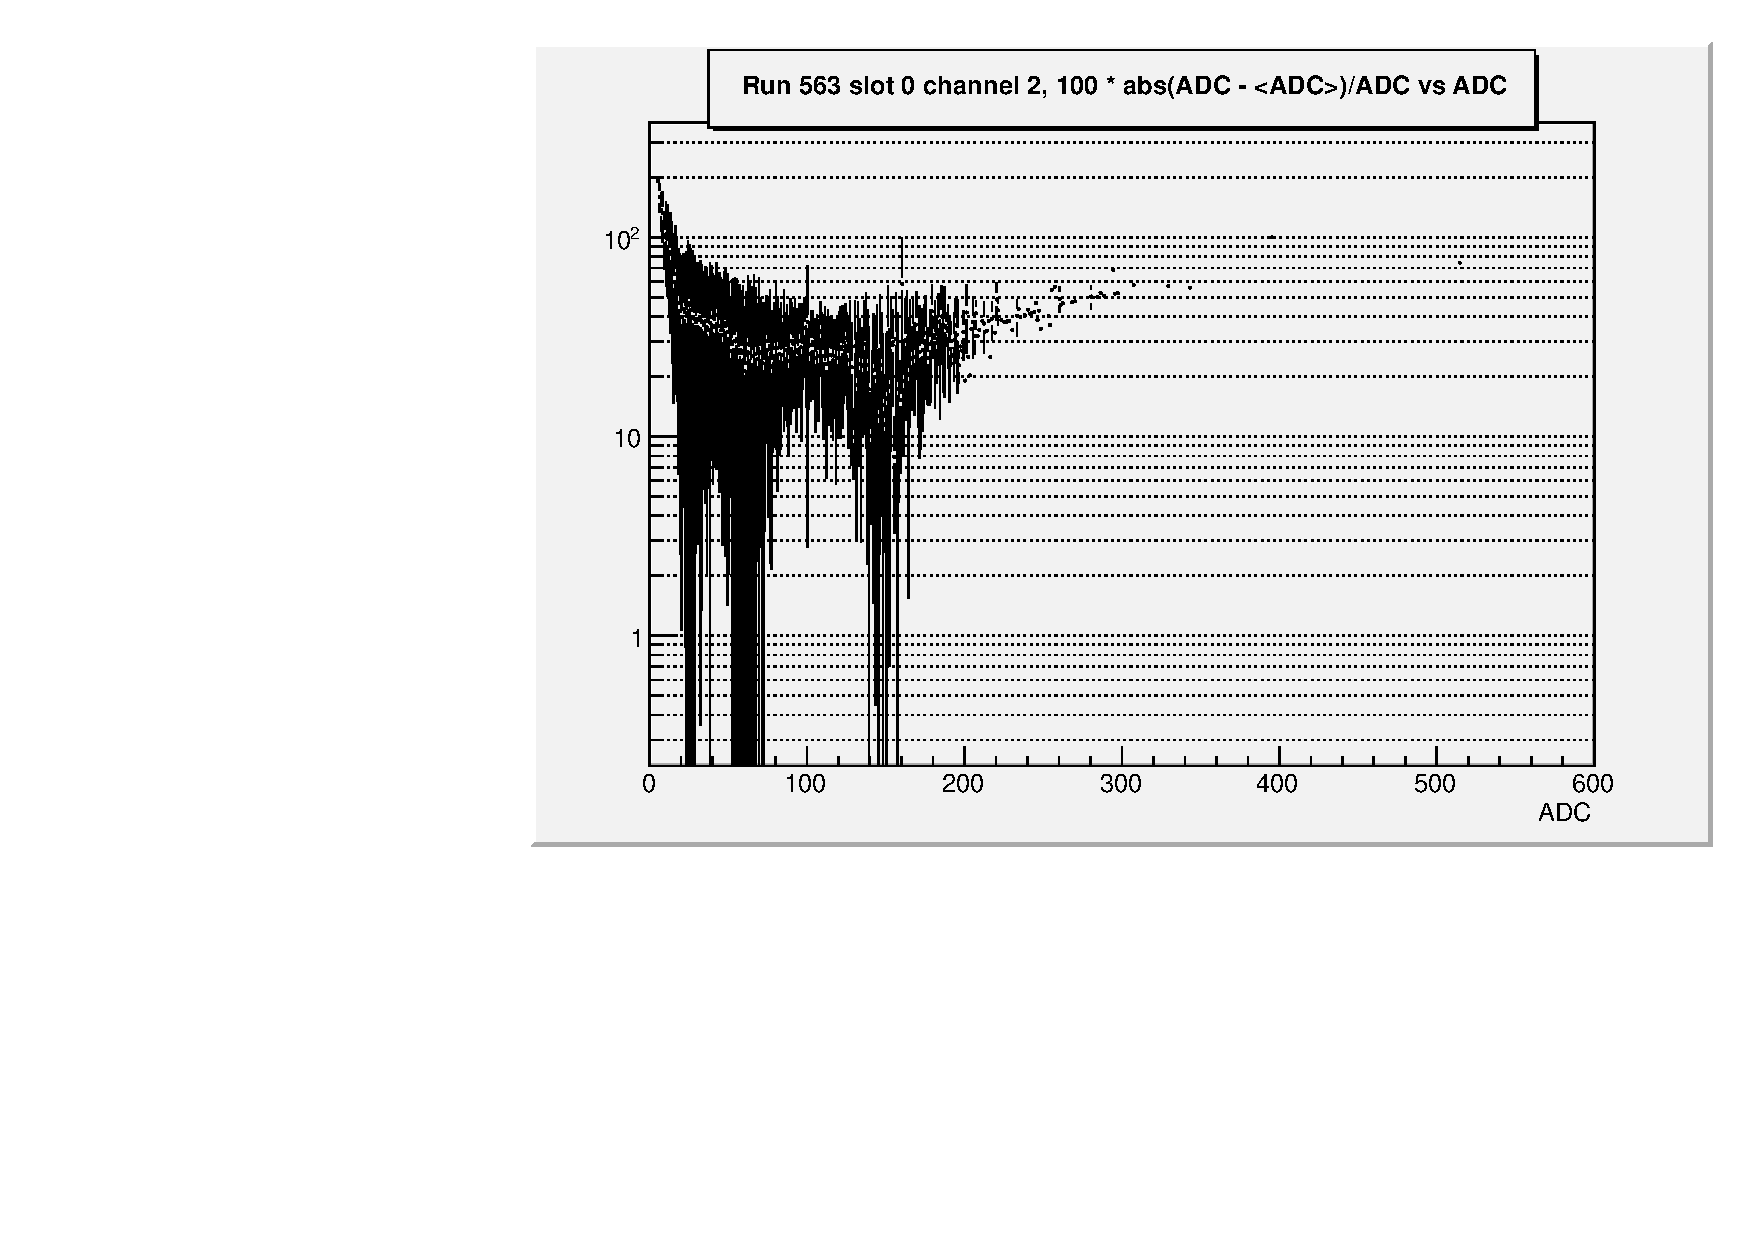
\includegraphics[width=\textwidth]{walk_NINO_1_4_PMT_700}
\caption{Walk for runs 536 (top figure, NINO threshold -1.9 V) and 563 (bottom figure, NINO threshold -1.4 V). 
Both figures represent slot 0 channel 2 in logarithmic scale, HV=-700V, NINO card 1, 324k events.
In the first case, most of the histogram is below 20\%, as opposed to 50\% of the second case.}
\label{fig:walk}
\end{figure}


\subsection{Frequency of noise}\label{sec:noise}
TODO.
freq vs Vth, freq = n/N/t where t=channels/2 ns, n (N) is number of events within 0-tdccut (no cut) respectively.

See figure \ref{fig:noise}

\begin{figure}[htbp]
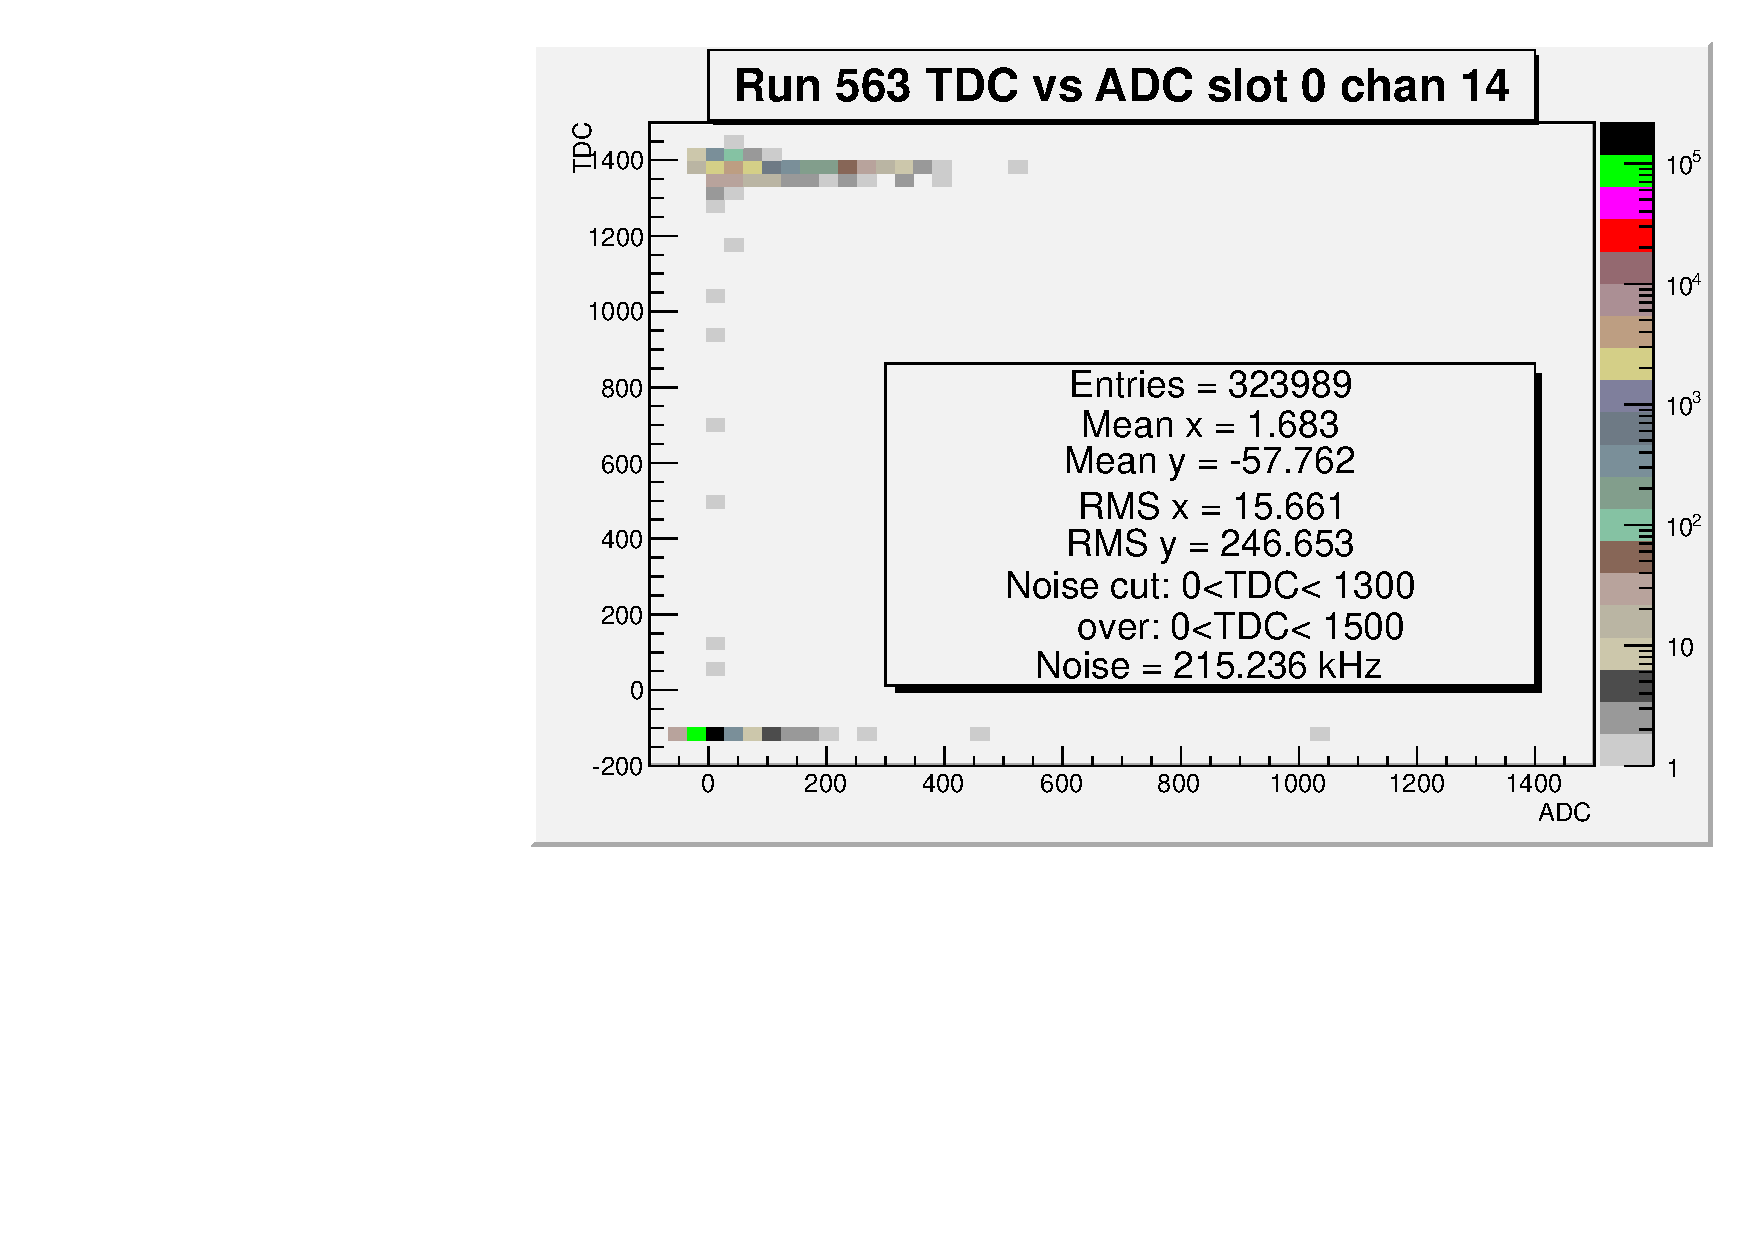
\includegraphics[width=\textwidth]{run_563_tdc_vs_adc_chan_14}
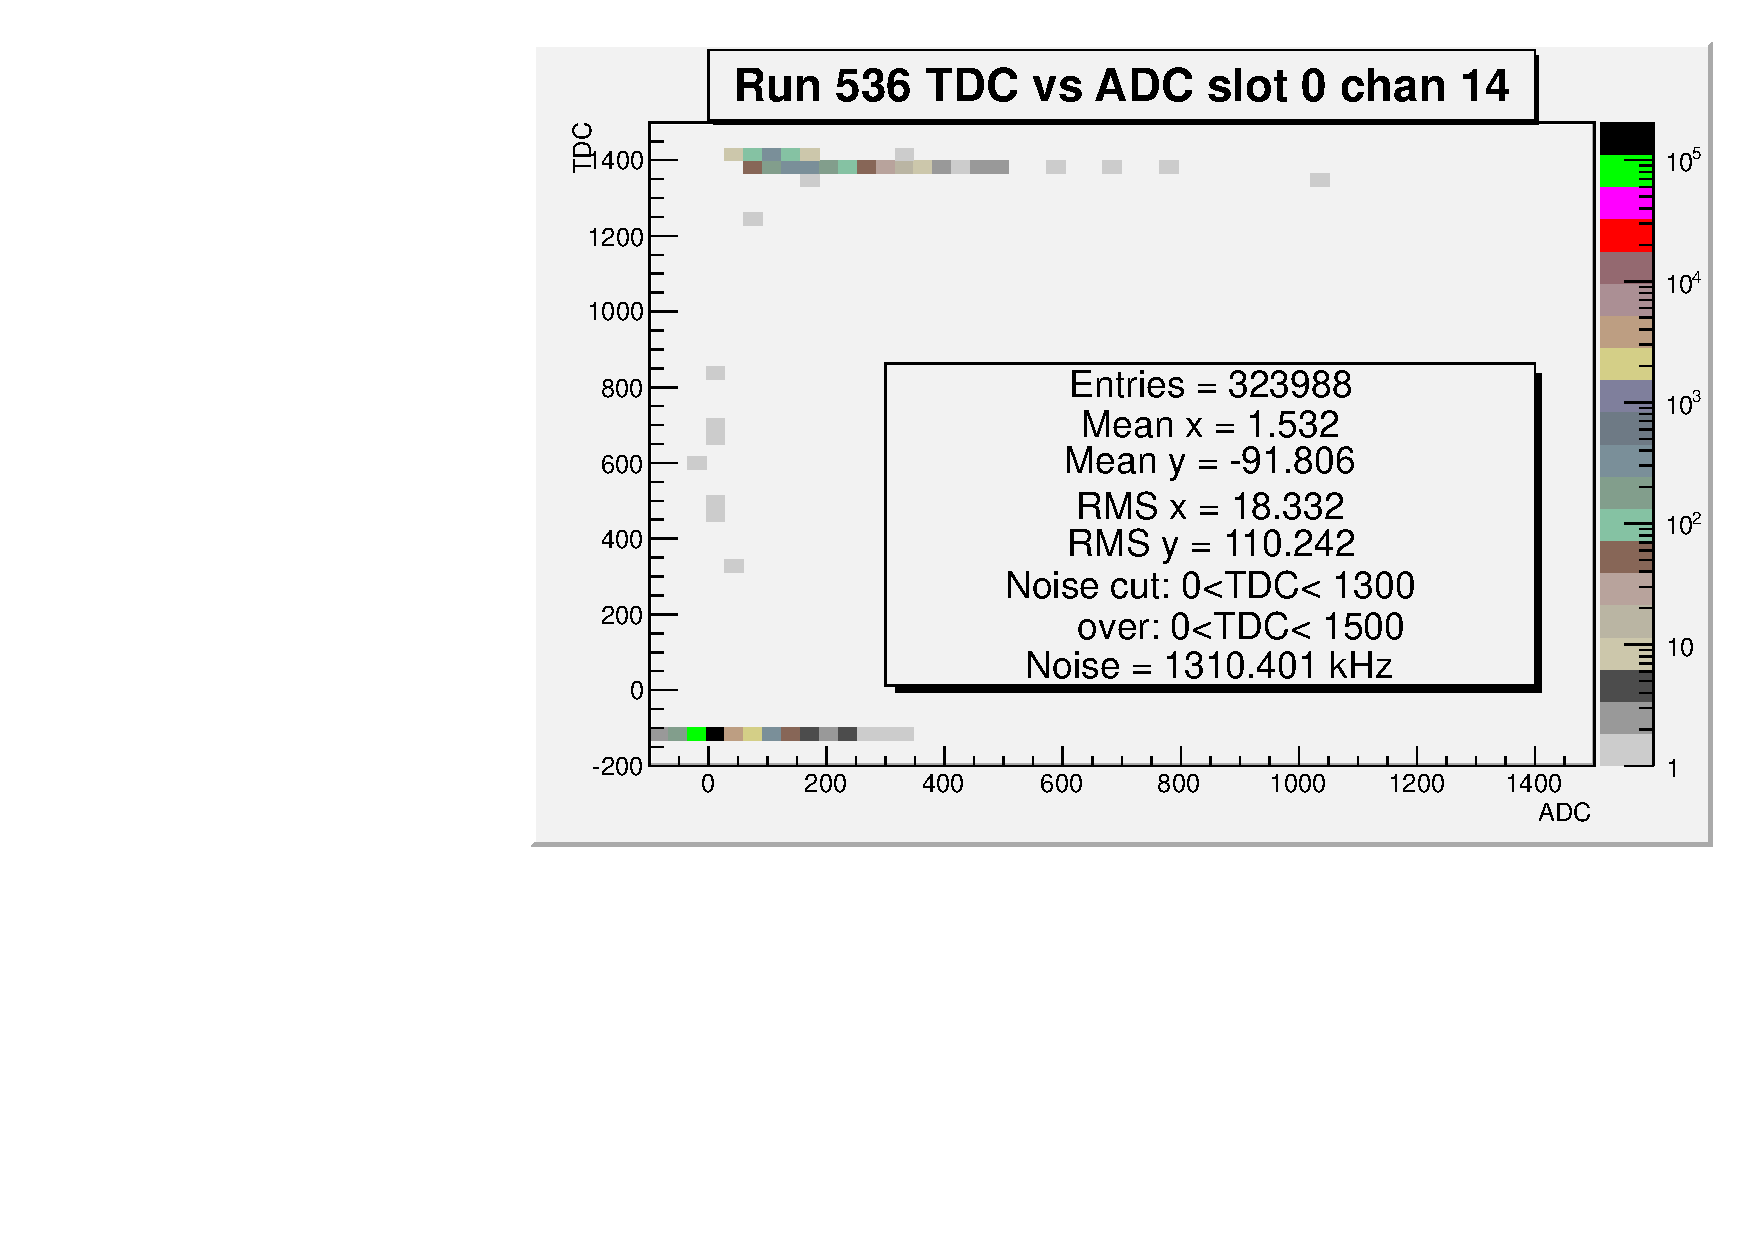
\includegraphics[width=\textwidth]{run_536_tdc_vs_adc_chan_14}
\caption{Noise frequency calculation for runs 563 and 536. The presented plots are relative to slot 0 channel 14. Both runs were acquired with HV=-700V, NINO card 1. The NINO thresholds are -1.4 V and -1.9V respectively.}
\label{fig:noise}
\end{figure}

\section{Analysis code}\label{sec:code}
SHOULD I TALK ABOUT IT AT ALL?


\begin{verbatim}
LIST OF FUNCTIONS in init.C

You may notice that most of the plot functions names may or may have
not a "1" at the end of the name.  The versions *with* the "1"
(e.g. plot_eta1) give a single plot, as opposed to the versions
*without* the "1" (e.g. plot_eta), which give a multiplot of 16
channels.



//
// RUN THIS FIRST!
//



init(runno)
// reads root file corresponding to run runno, extracts the tree with raw data,
// define shortcuts for slot 0 AT THE MOMENT, ONLY SLOT 0 CHANS 0-47 HAVE 
// SHORTCUTS!!!
// Note: in the general function section I added functions to convert slots and
// chans ADC from/to TDC. They are used in the plot_* routines, but I am not sure
// how to meaningfully use them for the following aliases



//
// PLOT_ functions
//



plot_eta1( adc_slot, adc_chan, tdc_cut, tdc_slot = -1, tdc_chan = -1, Ath_suggested=75, Aw_suggested=7)
// plot eta (calculated from histos) and its fit for a given slot and
// channel.
// Starting values for threshold and width may be suggested.
// The fit results are stored in global arrays Athresholds and Awidths

plot_eta( adc_slot, adc_chan_start, tdc_cut, tdc_slot = -1, tdc_chan_start = -1)
// plot 16 eta (calculated from histos) and its fit for a given slot
// and from a channel. The fit results are stored in global arrays Athresholds 
// and Awidths

plot_tdc( tdc_slot, tdc_chan_start, adc_cut, adc_slot = -1, adc_chan_start = -1)
// plot canvas divided in 4x4 TDC plots of 16 channels starting from
// adc_chan_start, of given slot. TDC is plotted with and without the
// following cut: adc value > adc_cut
// By default, tdc starting chan = adc starting chan; if passed a
// different value than -1 to adc_chan_start, that value will be used
// instead. May be useful during testing of ADC/TDC channels
// Analogously for adc_slot

plot_adc( adc_slot, adc_chan_start, tdc_cut, tdc_slot = -1, tdc_chan_start = -1
// plot canvas divided in 4x4 ADC plots of 16 channels starting from
// adc_chan_start, of given slot. ADC is plotted with and without the
// following cut: tdc value > tdc_cut
// By default, tdc starting chan and slot are calculated
// automatically; if a different values than -1 to
// tdc_chan_start/slot, those values will be used instead. May be
// useful during testing of ADC/TDC channels

plot_tdc_vs_adc(adc_slot, adc_chan_start, tdc_slot = -1, tdc_chan_start = -1){
// For interactive use: plot canvas divided in 4x4 TDC vs ADC plots of
// 16 channels starting from adc_chan_start, of given slot. No cuts.
// By default, tdc starting chan is calculated from adc starting chan;
// if passed a different value than -1 to tdc_chan_start, that value
// will be used instead. May be useful during testing of ADC/TDC
// channels. Fills global vector for noise freq

plot_peak1( slot, chan, value_lt=10, value_gt=100)
// plots the peak for vertical tracks for given slot/channel imposing
// the adjacent channels have counts < value_lt, and the chosen
// channel at least value_gt counts. Fills the global vectors

plot_peak( slot, chan_start, value_lt=10, value_gt=100)
// plots the peak for vertical tracks for 16 chans starting from given
// slot/channel imposing the adjacent channels have counts < value_lt,
// and the chosen channel at least value_gt counts. Fills the global vectors

plot_walk1(int adc_slot, int adc_chan, int tdc_slot=-1, int tdc_chan=-1, int adc_min=0, int adc_max=600, int deltat_min=0, int deltat_max=120, int stage=6)
// plots the walk correction of given adc(tdc) slot, channel, for adc
// in the range [adc_min, adc_max], and delta t (= leading edge -
// trailing edge) in range [deltat_min, deltat_max].
//
// The stage flag may be used to see various steps of the calculation:
// stage == 1 user wants to check raw data;
// stage == 2 user wants to see the profile histogram of stage 1;
// stage == 3 user wants to see the distribution of ADC - mean;
// stage == 4 user wants to see ADC-mean vs ADC;
// stage == 5 user wants to see (ADC-mean)/ADC vs ADC;
// stage == 6 same as stage == 5, but profile



//
// AUXiliary functions. Normally there is no reason to call them
// interactively
//



noise_freq(tdc_slot, tdc_chan, tdc_cut)
// calculate the noise frequency (in Hz) for given tdc slot, chan, cut

phe(adc_slot, adc_chan)
// Calculate the number of phe for a given adc slot, chain

gain(adc_slot, adc_chan)
// calculate gain for a given adc slot, chan

calc_adc_chan( tdc_slot, tdc_chan)
// find the adc slot corresponding to a given tdc slot/channel

calc_adc_slot( tdc_slot, tdc_chan)
// find the tdc slot corresponding to a given tdc slot/channel

calc_tdc_chan( adc_slot, adc_chan)
// find the tdc chan corresponding to a given adc slot/channel

calc_tdc_slot( adc_slot, adc_chan)
// find the tdc slot corresponding to a given adc slot/channel

fit_eta_in_slot( adc_slot=0, adc_chan_min=0, adc_chan_max=63, tdc_cut=1200, tdc_slot = -1, tdc_chan = -1)
// auxiliary function. Calculate all eta fits for slot, between
// chan_min and chan_max (inclusive), in order to populate the
// arrays. Used in save_eta()

peak_rms( slot, chan, value_lt=10, value_gt=100)
// find the RMS of the peak for a given slot/channel imposing the
// adjacent channels have counts < value_lt, and the chosen channel
// at least value_gt counts

peak_mean( slot, chan, value_lt=10, value_gt=100)
// find the position of the peak for a given slot/channel imposing the
// adjacent channels have counts < value_lt, and the chosen channel
// at least value_gt counts

save_data(abs_NINOthreshold_V, abs_PMT_HV_V, 
	       adc_slot=-1, chan_min=0, chan_max=63, 
	       tdc_slot=-1, tdc_chan=-1)
// For interactive use:
// save results (retrieved from global arrays, see "format" variable for
// details) on a file named after run number, NINO threshold and PMT
// voltage (overwrite mode).
// Default values meaning:
// save every ADC slot (slot = -1), every ADC channel (0,63). 
// TDC slot/chan are calculated from ADC ones.
\end{verbatim}

\textbf{EDIT END}



\end{document}
